% CVSId: $Id: Example.tex,v 1.1.1.1 2000/11/28 11:15:12 exupery Exp $
\documentclass[%
xcolor=pdftex,dvipsnames,table%,
%pdf,
%nocolorBG,
%colorBG,
%slideColor,
%slideBW,
%draft,
%frames
%azure
%contemporain
%nuancegris
%troispoints
%lignesbleues
%darkblue
%alienglow
%autumn
%10pt
]{beamer}
\usepackage[absolute,overlay]{textpos}
%%%%%%%%%%%%%%%%%%%%%%%%%%%%%%
%Force pdflatex processing even with "$ latex" (required by arXiv)
\pdfoutput=1
%%%%%%%%%%%%%%%%%%%%%%%%%%%%%
\mode<presentation>
{
  %\usetheme{Madrid}
  \usetheme{Boadilla}
  % or ...
%%%%%%%%%%%%%%%%%%%%%%%%%%%%%%%%%%%%%
%para revelar texto a aparecer en overlays
  %\setbeamercovered{transparent} 
  %\setbeamercovered{invisible}
%%%%%%%%%%%%%%%%%%%%%%%%%%%%%%%%%%%%%
  \setbeamertemplate{blocks}[rounded][shadow=true]
  \setbeamertemplate{navigation symbols}{}

  \setbeamertemplate{footline}{%\hspace*{.5cm}
    \scriptsize{\phantom{Gg}%\insertauthor 
      \hspace*{50pt} 
      \hfill \insertframenumber
      \hspace*{.5cm}}}

  % or whatever (possibly just delete it)
  %\useoutertheme{shadow} 
  \setbeamercolor{postit}{fg=black,bg=yellow}
  \setbeamercolor{white}{fg=black,bg=white}
  \setbeamercolor{cite}{fg=black,bg=yellow}
}
\graphicspath{{figures/}}
\usepackage[T1]{fontenc}
\usepackage[utf8]{inputenc}
\usepackage[spanish]{babel}
\spanishdecimal{.}
\usepackage{marvosym}
\usepackage{beamerprosper}
\usepackage{amsmath,amssymb}
\usepackage{graphicx}
\usepackage{mycolors}
\usepackage{xmpmulti}
\usepackage{multimedia}
\usepackage{pgf}
\usepackage{cancel}
\usepackage{comment}
\includecomment{comentar}
\specialcomment{comentar}
{\begingroup}{\medskip\endgroup}
\excludecomment{comentar}

\includecomment{comentario}
\specialcomment{comentario}
{\begingroup}{\endgroup}
\excludecomment{comentario}

\includecomment{details}
\specialcomment{details}
{\begingroup}{\endgroup}
\excludecomment{details}

%\usepackage[texcoord,grid,gridunit=mm,gridcolor=red!10,subgridcolor=green!10]{eso-pic}


\newcommand{\widescreen}{
\setlength{\paperwidth}{171 mm}
\setlength{\paperheight}{96 mm}
\setlength{\textwidth}{161 mm}
\setlength{\textheight}{86 mm}
}

%\widescreen


\title[RE] % (optional, use only with long paper titles)
{Dark matter realization of the Weinberg neutrino mass operator}

%\subtitle
%{Reconstruction of the neutrino mass matrix} % (optional)

\author[GFIF]% (optional, use only with lots of authors)
{Diego Restrepo\inst{1} }
% - Use the \inst{?} command only if the authors have different
%   affiliation.

\institute[UdeA] % (optional, but mostly needed)
{
  \inst{1}%
Instituto de F\'\i sica\\
Universidad de Antioquia\\
Phenomenology Group (\alert{GFIF: 4+1+4+2+$\cdots$})\\
\url{http://gfif.udea.edu.co}
\quad\\
\quad\\
\alert{\textbf{Focus on}} \\
arXiv:1308.3655\\
\alert{In collaboration with}\\
  Carlos Yaguna (M\"unster University)
\&\ Oscar Zapata (UdeA)
}
% - Use the \inst command only if there are several affiliations.
% - Keep it simple, no one is interested in your street address.

\date[] % (optional)
{
\includegraphics[scale=0.3]{udea}}


\subject{Talks}
% This is only inserted into the PDF information catalog. Can be left
% out. 



% If you have a file called "university-logo-filename.xxx", where xxx
% is a graphic format that can be processed by latex or pdflatex,
% resp., then you can add a logo as follows:

% \pgfdeclareimage[height=0.5cm]{university-logo}{university-logo-filename}
% \logo{\pgfuseimage{university-logo}}



% Delete this, if you do not want the table of contents to pop up at
% the beginning of each subsection:
%\AtBeginSubsection[]
%{
%  \begin{frame}<beamer>
%    \frametitle{Outline}
%    \tableofcontents[currentsection,currentsubsection]
%  \end{frame}
%}

\newcommand{\chml}[2]{$\underline{\text{#1\hspace{#2}}}$}
\begin{document}


%===============
\begin{comentar}
%===============  
%=============
\end{comentar}
%=============

\begin{frame}[plain]
\begin{picture}(320,250)
\only<1>{\put(-10,-5){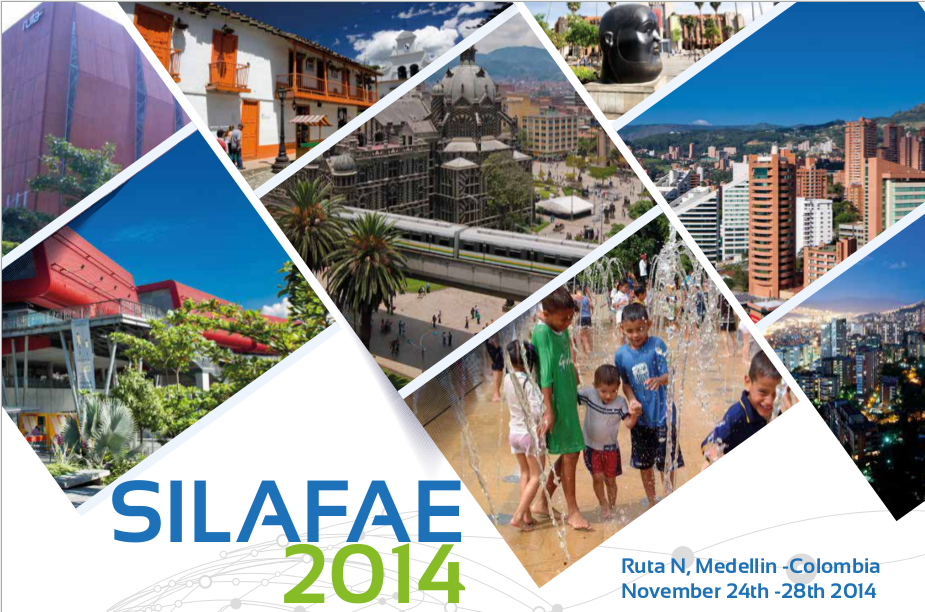
\includegraphics[scale=0.52]{silafae1}}}%
\only<2>{\put(-10,50){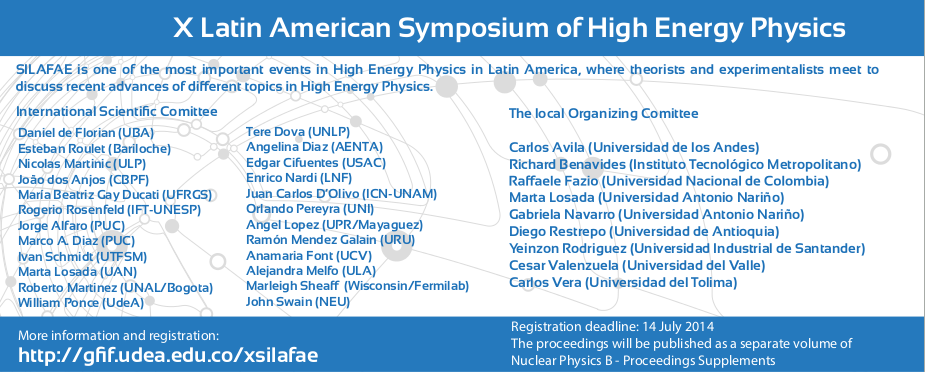
\includegraphics[scale=0.52]{silafae2}}}%
\only<2>{\put(-10,40){
   \begin{minipage}[t]{10cm}
 \tiny \color{blue}Scientific secretariat (UdeA):\\
 Dilia Portillo\\
 Marta Sánchez\\
 Camilo Salazar\\      
\vspace{0.5cm}
Avalaibe finanancial help for students and youth researchers
    \end{minipage}
}}%
\only<3>{\put(-10,30){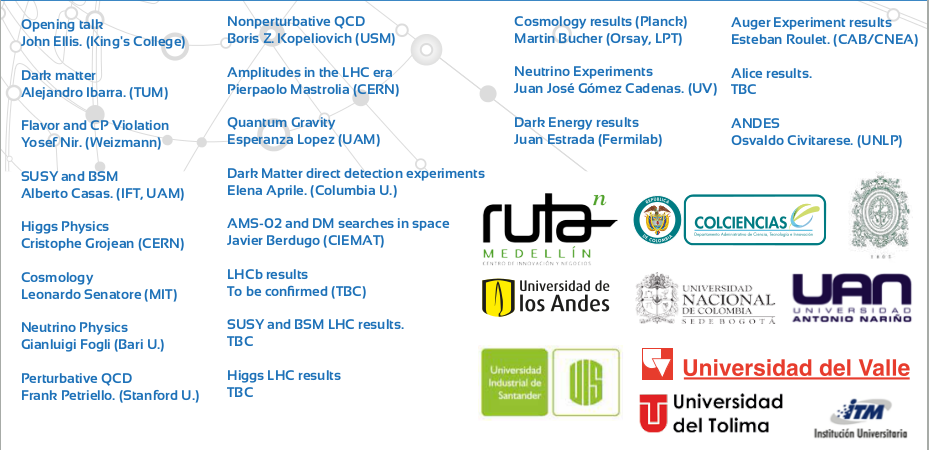
\includegraphics[scale=0.52]{silafae3}}}%
\end{picture}
\end{frame}

% {
% \setbeamertemplate{background}{
\includegraphics[width=\paperwidth]{gfif_bkg}}
 \begin{frame}[plain]
   \titlepage
 \end{frame}
% }



% {
% \usebackgroundtemplate{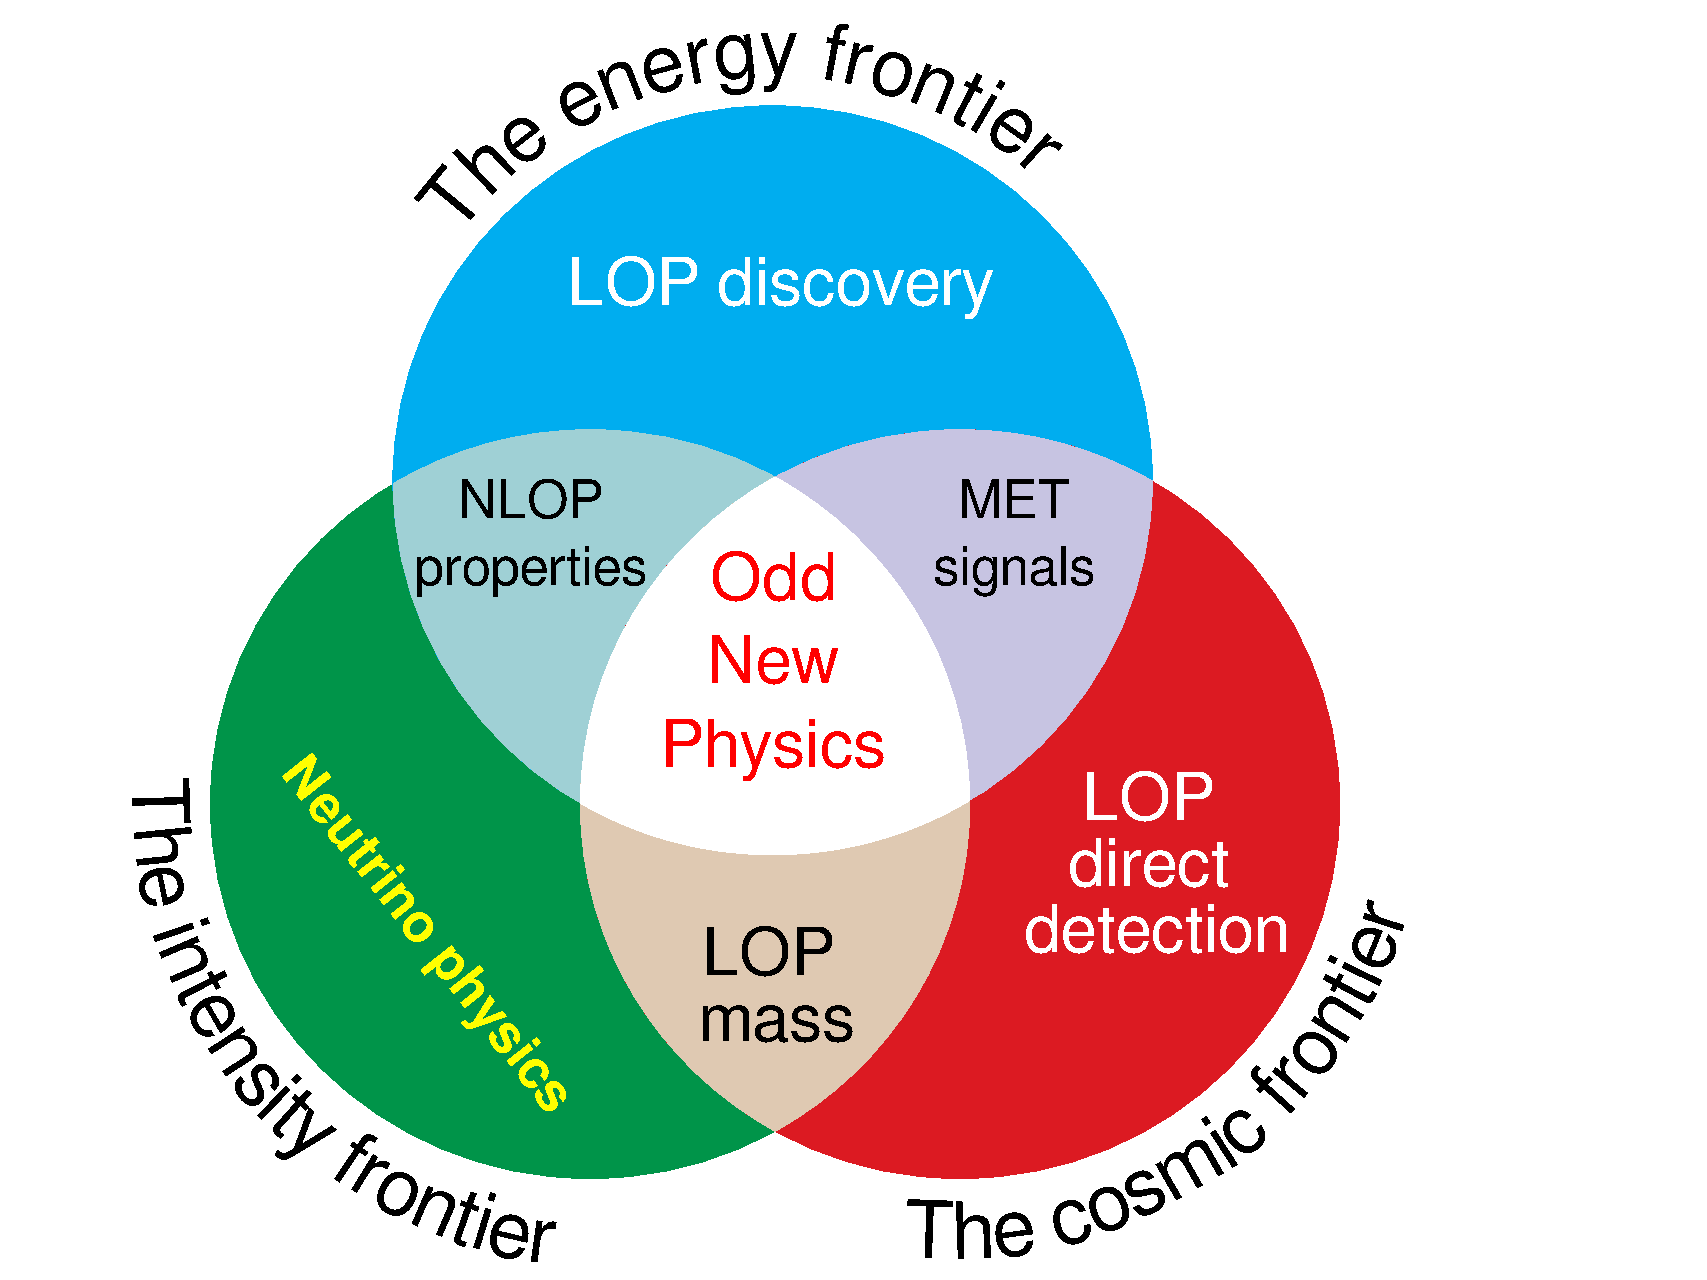
\includegraphics[width=\paperwidth]{tocrs}}
\begin{frame}
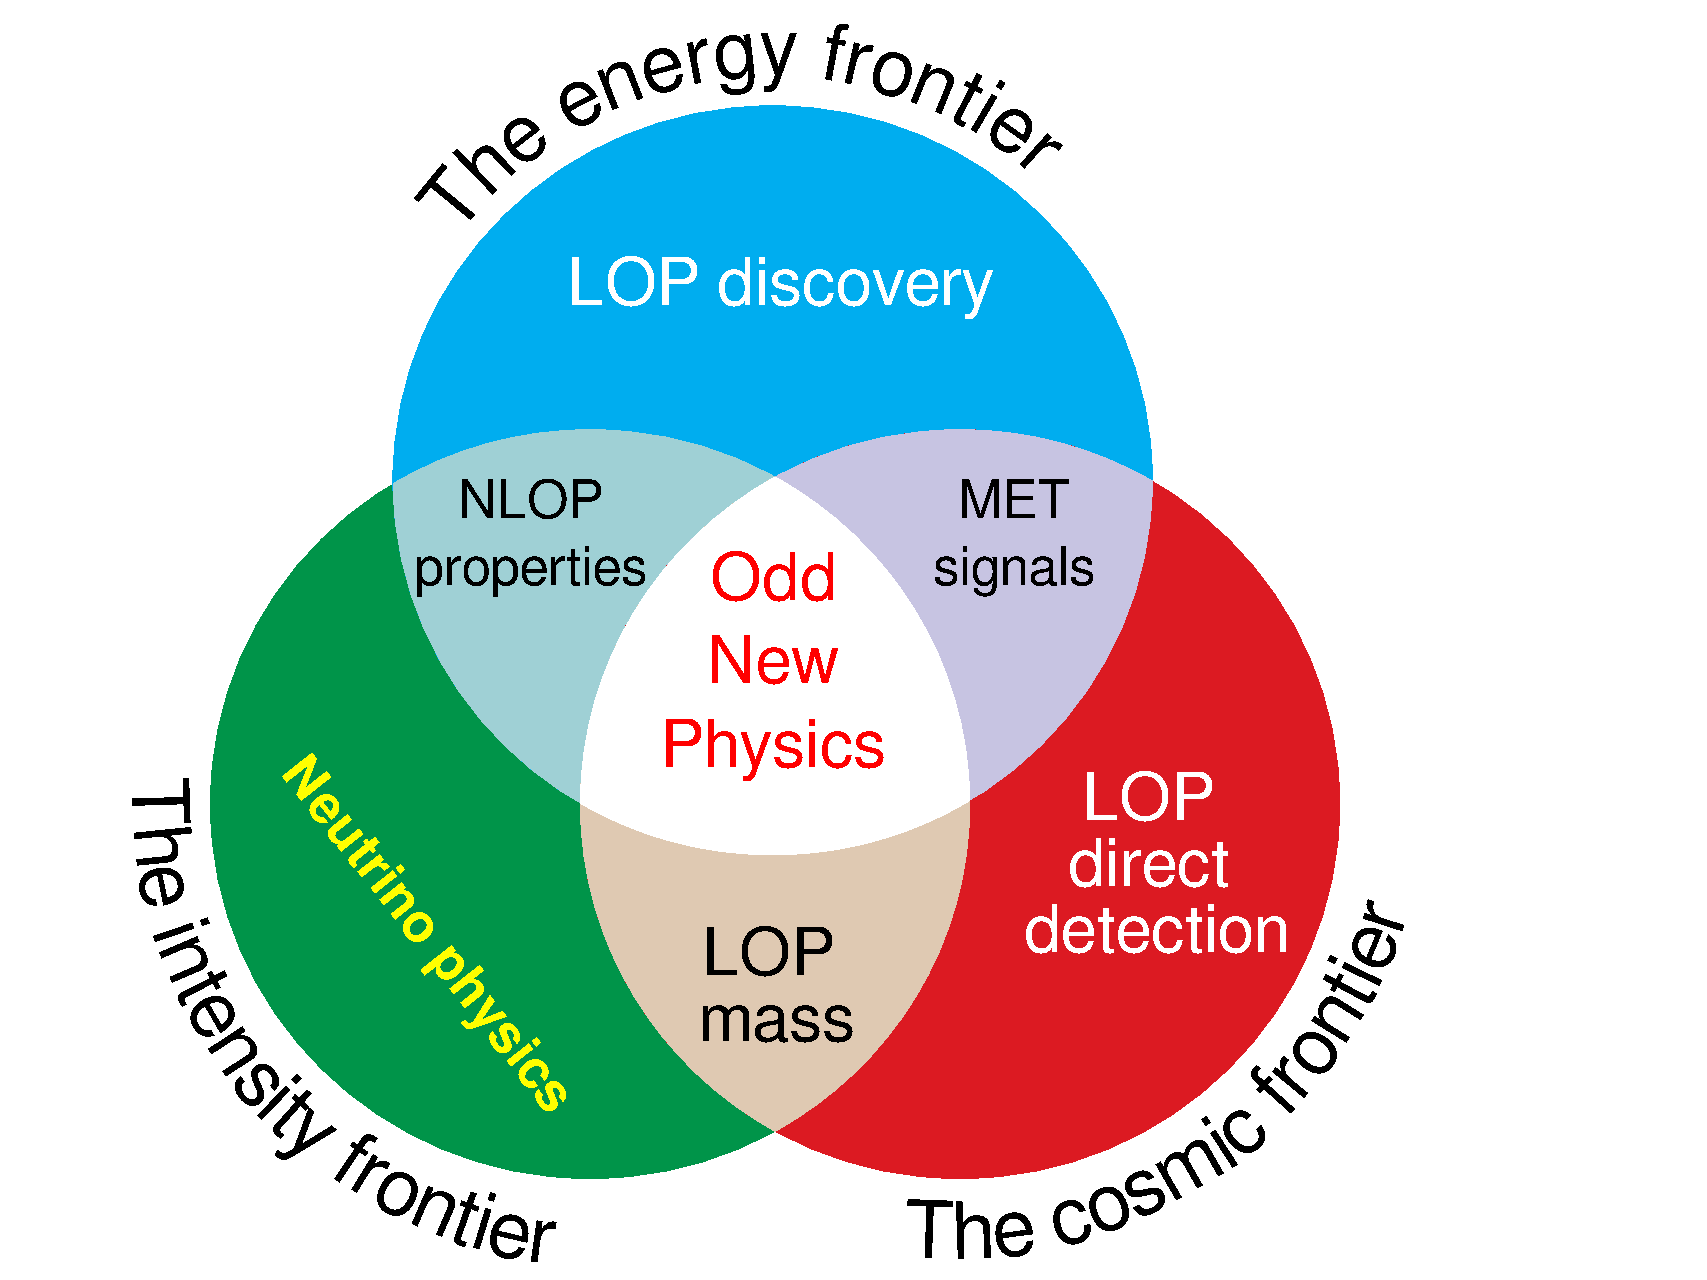
\includegraphics[scale=0.38]{tocrs}
 %   \begin{picture}(320,250)
 % \only<1->{\put(-11,10){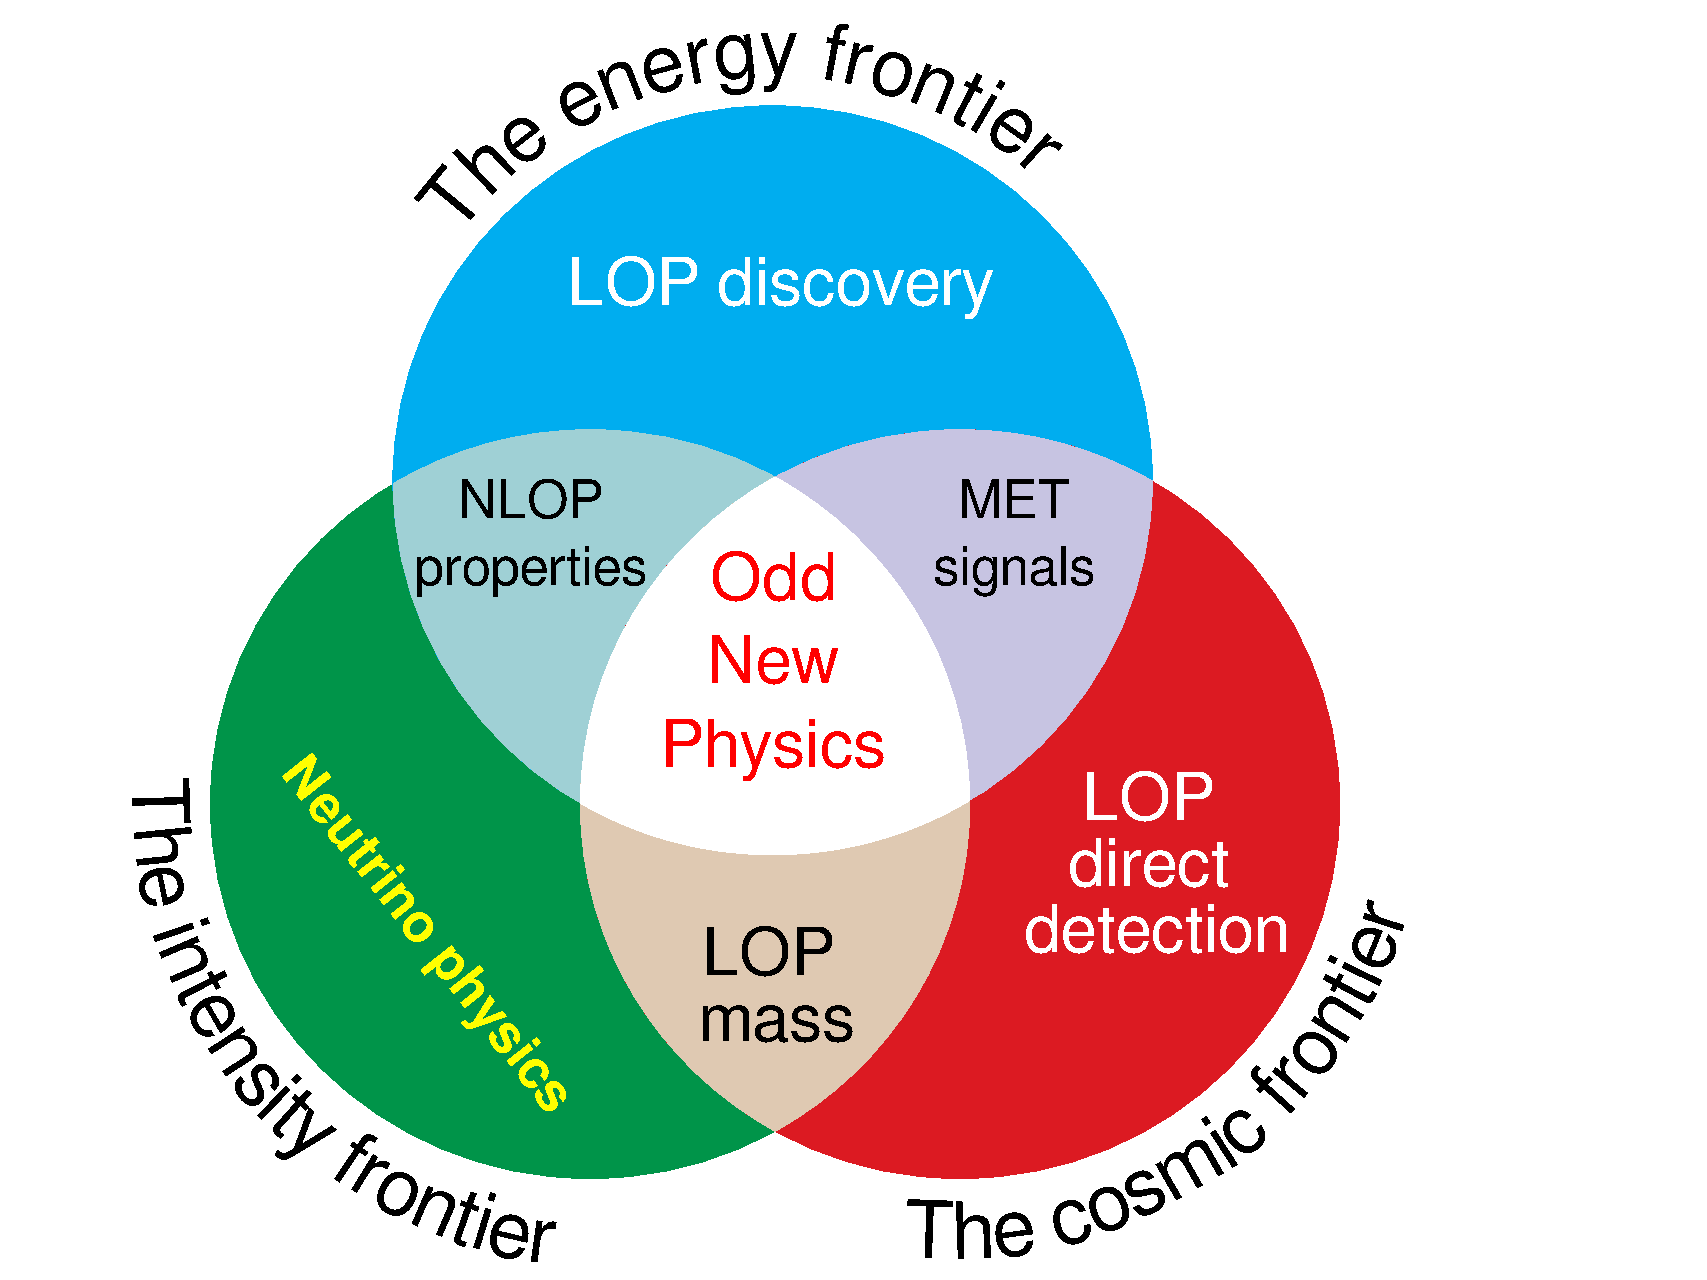
\includegraphics[scale=0.4]{tocrs}}}%
 % \end{picture}

 Standard Model $Z_2$-Even particles + \alert{New $Z_2$-Odd new particles}

 \alert{Lightest Odd Particle (LOP)} may be  a suitable dark matter candidate
\end{frame}
% }


\begin{frame}
\begin{picture}(320,250)
\only<1->{\put(-11,210){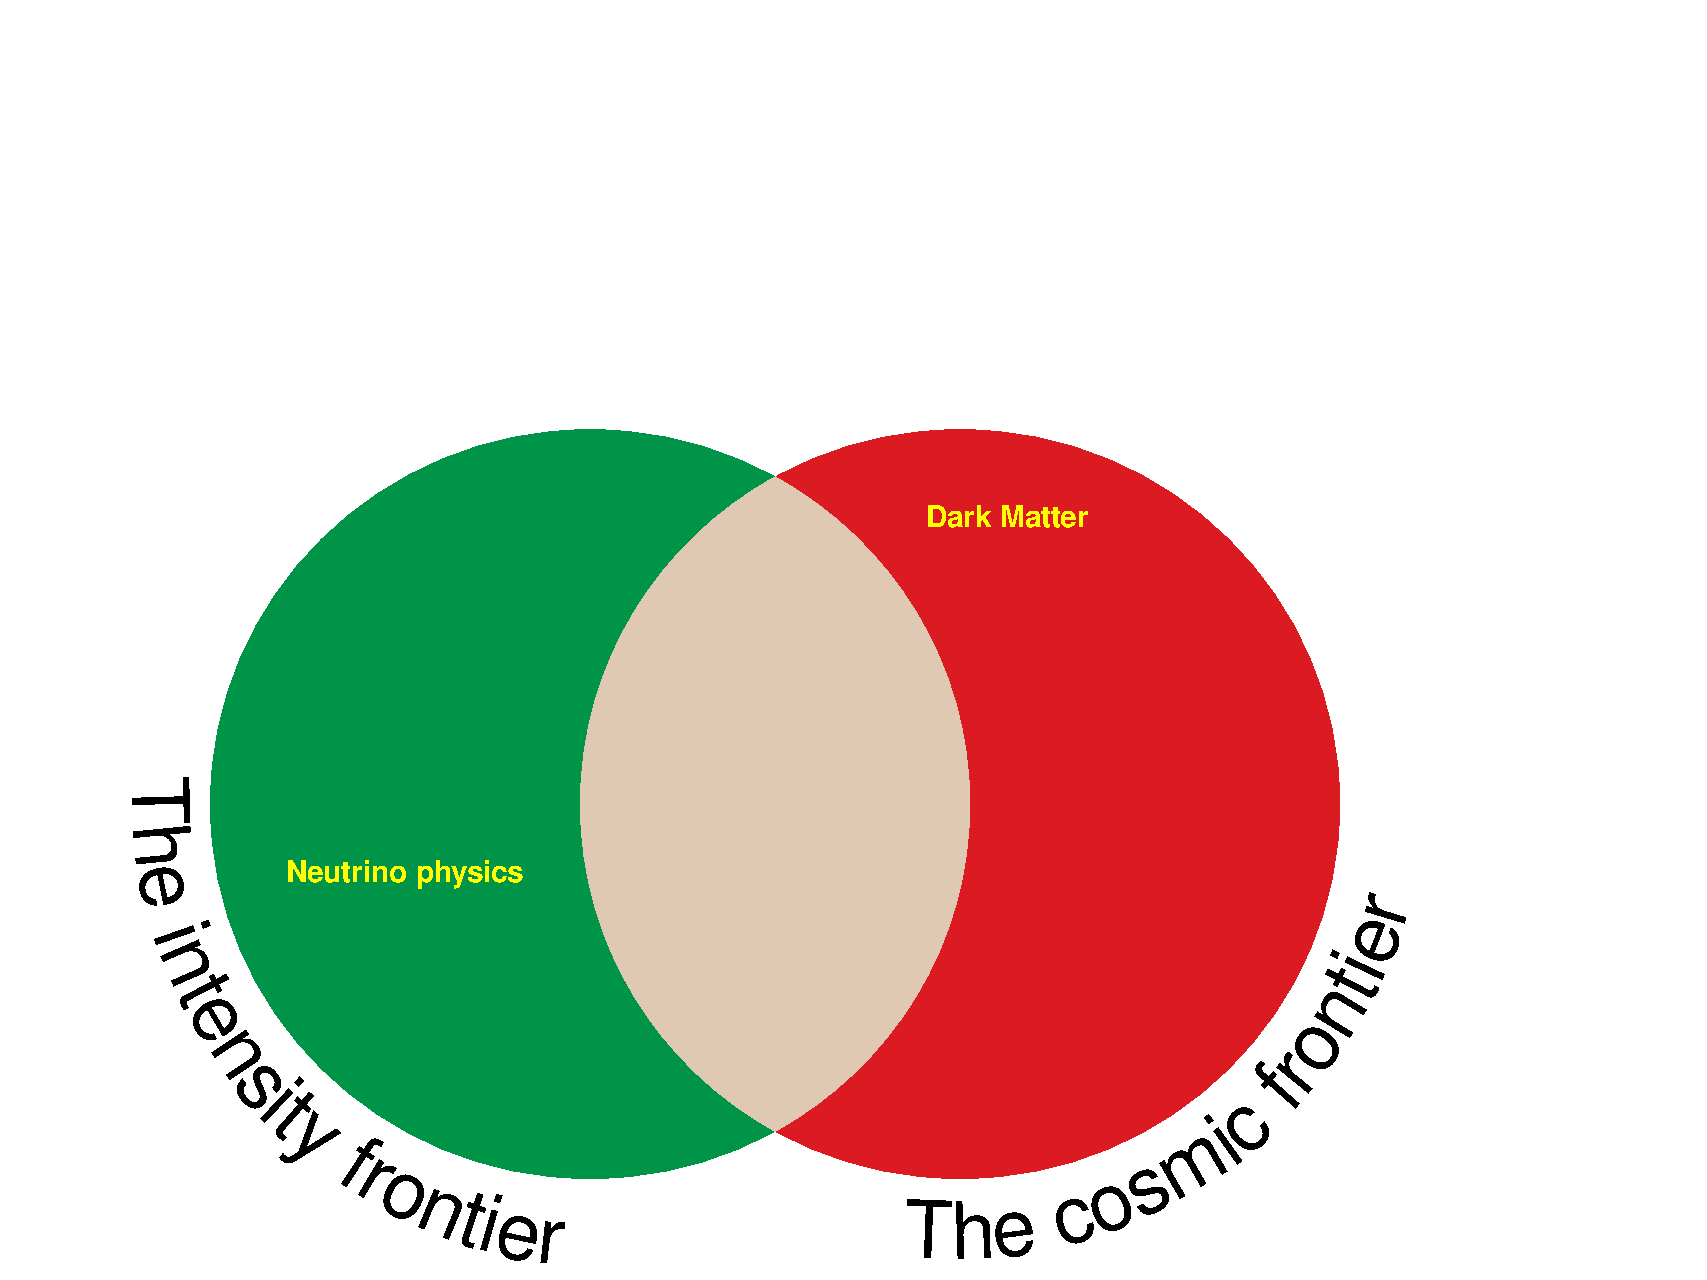
\includegraphics[scale=0.1]{tfIClarge}}}%
\only<1>{\put(-11,45){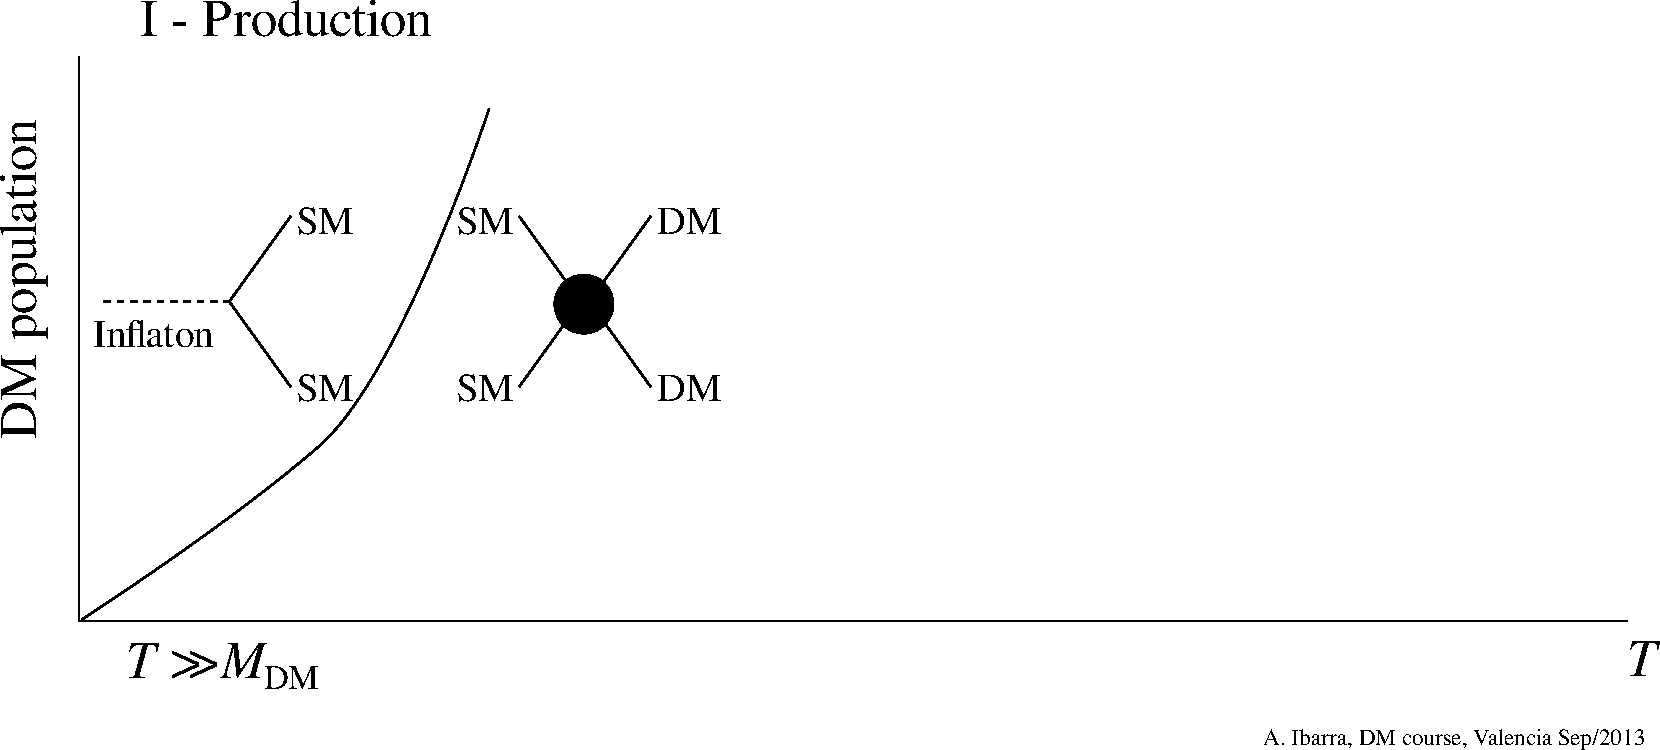
\includegraphics[width=\paperwidth]{earlyuniverse1}}}%
\only<2>{\put(-11,45){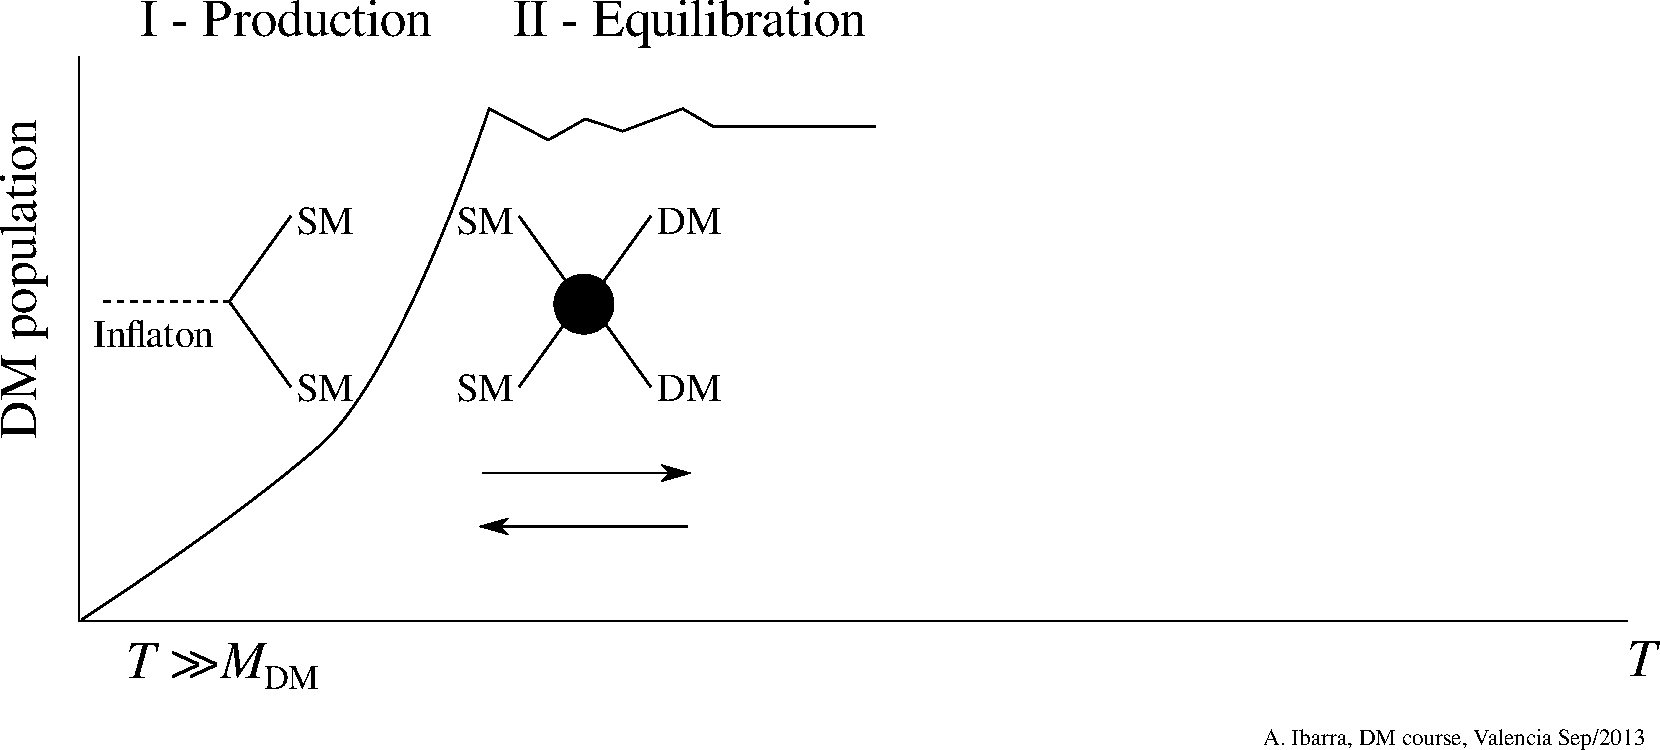
\includegraphics[width=\paperwidth]{earlyuniverse2}}}%
\only<3>{\put(-11,45){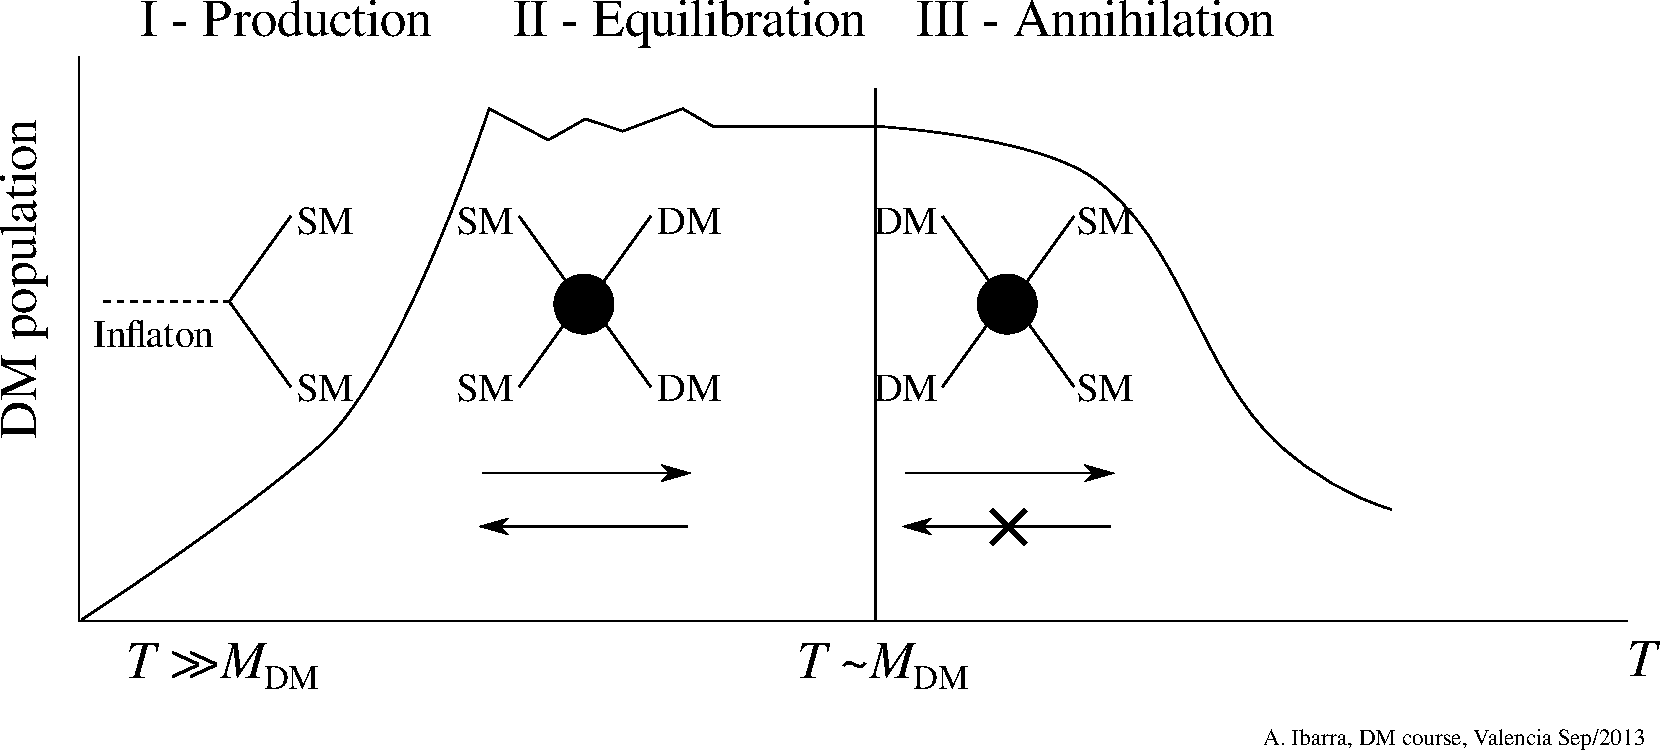
\includegraphics[width=\paperwidth]{earlyuniverse3}}}%
\only<4->{\put(-11,45){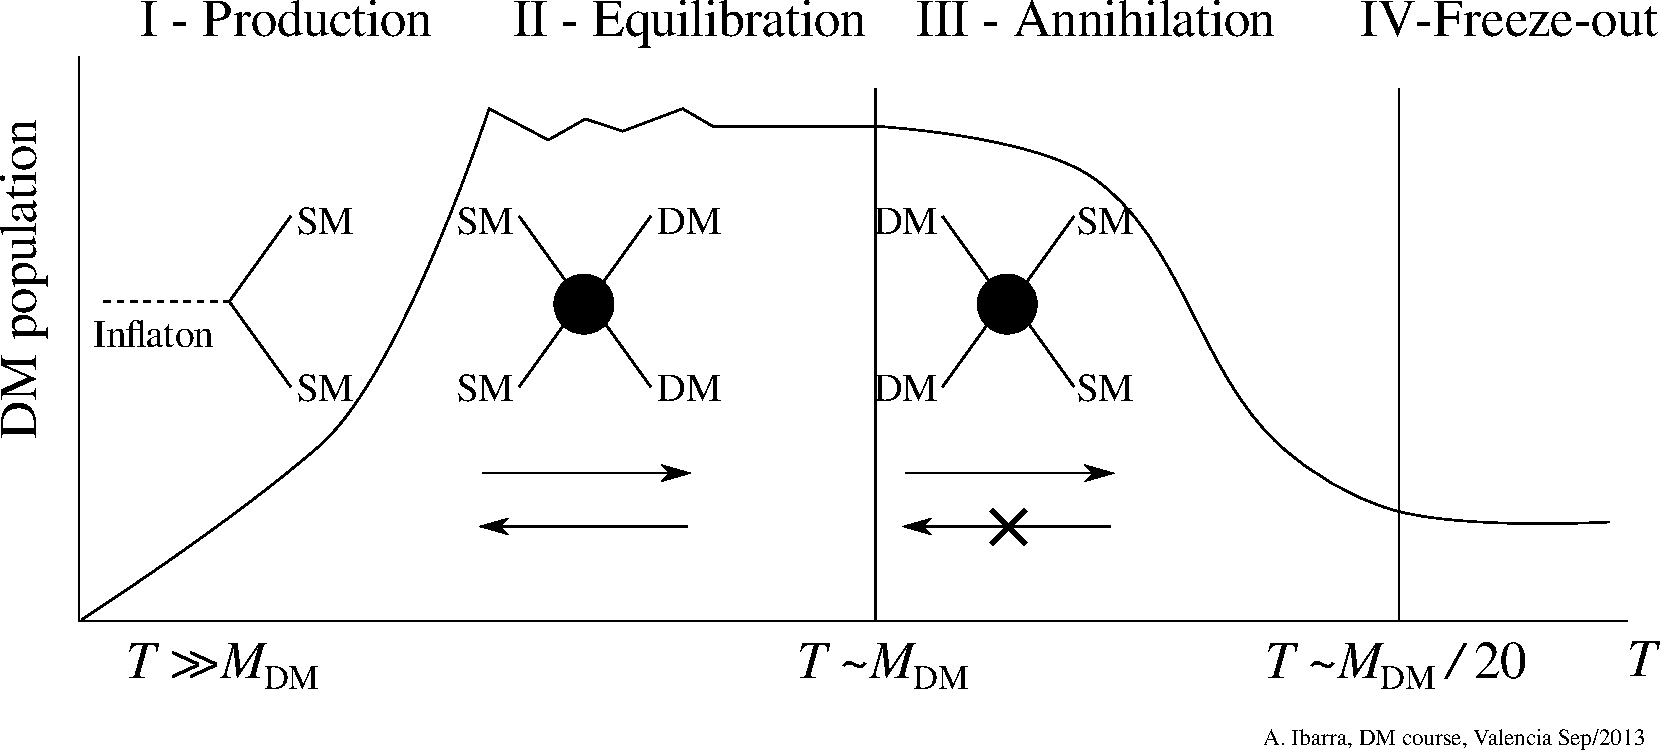
\includegraphics[width=\paperwidth]{earlyuniverse4}}}%
\only<5>{\put(-11,10){
    \begin{minipage}{0.5\linewidth}
      \rowcolors{1}{RoyalBlue!20}{}
\begin{tabular}{ll}
  Parámetro& $1\sigma$ \\\hline
 $\Delta m^{2}_{32}[10^{-3}\mathrm{eV^{2}}]$ & $2.50^{+0.09}_{-0.16}$ \\
  $\Delta m^{2}_{21}[10^{-5}\mathrm{eV^{2}}]$ & $7.59^{+0.20}_{-0.18}$ \\
\end{tabular}\\
    \end{minipage}
    \begin{minipage}{0.5\linewidth}
      \rowcolors{1}{RoyalBlue!20}{}
\begin{tabular}{ll}
  Parámetro& $1\sigma$ \\\hline
  $\sin^{2}{\theta_{23}}$ & $0.52^{+0.06}_{0.07}$ \\
  $\sin^{2}{\theta_{12}}$ & $0.312^{+0.017}_{-0.015}$ \\
  $\sin^{2}{\theta_{13}}$ & $0.013^{+0.007}_{-0.005}$ \\
\end{tabular}\\
    \end{minipage}
}}

\end{picture}
\end{frame}
%%%%%%%%%%%%%%%%%%%%
\begin{frame}
\frametitle{Electroweak searches}
No new physics with strong production at LHC Run-I.

Many possibilities for new physics with EW production. 

For example: SM $SU(2)_L$-triplet fermion with zero hypercharge: $\boldsymbol{\Sigma}_0$ (or $\widetilde{\boldsymbol{W}}$ in SUSY)

\rowcolors{1}{RoyalBlue!20}{}
\begin{tabular}{p{3.5cm}|p{4cm}|p{3.5cm}}
Not large missing $E_T$&\multicolumn{2}{c}{Large missing $E_T$} \\\hline
Type-III Seesaw & Simplified SUSY model with only $M_1, M_2$ below 1~TeV and $M_1<M_2$ & Scotogenic Type-III Seesaw\\\hline
CMS arXiv:1207.6079 &CMS arXiv:1309.7509&In progress (see Poster Session) \\
$pp\to \Sigma^\pm \Sigma^0 $&$pp\to \tilde{\chi}_1^\pm\tilde{\chi}_2^0$&$pp\to \Sigma^{\pm}+ \Sigma^0 $\\
$\Sigma^\pm\to Z l^\pm$ &$\tilde{\chi}_{1}^\pm\to W^{\pm} \alert{\tilde{\chi}_1^0}$&$\Sigma^\pm\to \alert{H^0} l^\pm$\\ 
$\Sigma^0\to W^\pm l^{\mp}$&$\tilde{\chi}_{2}^0\to Z \alert{\tilde{\chi}_1^0}$&$\Sigma^0\to H^\pm l^{\mp}$\\
$W^{\pm}\to l^{\pm}\nu $ &$W^{\pm}\to l^{\pm}\nu $&$H^{\pm}\to W^{\pm} \alert{H^0} $\\
$(Z\to jj,\nu\nu)$ & $Z\to l^{\pm}l^{\mp}$&$W^{\pm}\to l^{\pm}\nu $\\
Trilepton &\multicolumn{2}{c}{Trilepton + $\cancel{E_T}$}\\
Neutrinos &\alert{DM?}& Neutrinos + \alert{DM}\\
\end{tabular}
\end{frame}
%%%%%%%%%%%%%%%%%%%%%%%
\begin{frame}
  \frametitle{Radiative type-I seesaw}
\begin{textblock*}{297mm}(60mm,0.5mm)%
\begin{beamercolorbox}[sep=0.01em,wd=6cm,center,rounded=true,shadow=true]{cite}
\scriptsize E. Ma, hep-ph/0601225 (PRD)
\end{beamercolorbox}
\end{textblock*}
\begin{textblock*}{297mm}(5mm,10mm)%
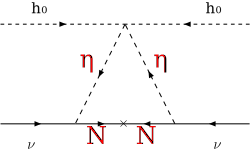
\includegraphics[scale=0.75]{rs}
\end{textblock*}
\begin{picture}(320,250)
\only<2->{\put(0,150){\parbox[t]{5cm}{\scriptsize
\begin{align*}
\color{red}
 \left(m_\nu\right)_{\alpha\beta}\simeq&\color{red} \sum_{i=1}^3\frac{2 \lambda_5 h_{\alpha i}h_{\beta i} v^2}{(4\pi)^2 M_i} I\left(\frac{M_i^2}{M_0^2}\right),\\
\color{red} I(x)=&\color{red}\frac{x}{1-x}\left(1+\frac{x\log x}{1-x}\right)\\
\color{red}M_0^2\simeq &\color{red}\mu_{2}^2+(\lambda_3+\lambda_4) v^2
\end{align*}
}}}
\only<1->{
\put(160,260){\parbox[t]{4cm}{
\begin{align*}
 -\mathcal{L} \supset&\frac{M_i}{2}\bar N_i^cP_RN_i-h_{\alpha i}\bar \ell_\alpha \eta^\dagger P_RN_i+\text{h.c.},\\
&+ \mu_{2}^2 \eta^\dagger \eta+\lambda_3 \left(H^\dagger H\right)\left(\eta^\dagger \eta \right)\\
&+\lambda_4\left(H^\dagger \eta\right)\left(\eta^\dagger H\right)\\
&+\frac{\lambda_5}{2}\left(H^\dagger \eta\right)^2
+\text{h.c.},\nonumber
\end{align*}}}
\put(180,150){\parbox[t]{5cm}{
\begin{align*}
 M_{H^{\pm}}^2&= \mu_2^2+\lambda_3v^2 ,\nonumber \\
\color{red}M_{H^0}^2&= \mu_2^2+(\lambda_3+\lambda_4+\lambda_5)v^2 ,\nonumber \\
M_{A^0}^2&= \mu_2^2+(\lambda_3+\lambda_4-\lambda_5)v^2\,, 
\end{align*}
}}
}
\only<3>{\put(10,70){\parbox[t]{5cm}{%\scriptsize
\begin{align*}
100~\text{GeV} &< {\color{red}M_{H^0}}<1~\text{TeV}&
 M_{H^0} &<  M_{A^0}< M_{H^0}+40~\text{GeV}\\
 M_{H^0} &<  M_{H^\pm}< M_{H^0}+40~\text{GeV}&
 M_{H^0} &< M_{N_i}<M_{H^0}+40~\text{GeV}\\
10^{-5} &< \lambda<10^{-1}&
10^{-6} &< h_2<10^{-1}\,.
\end{align*}
}}}
\end{picture}
  
\end{frame}

%%%%%%%%%%%%%%%%%%%%%%%%%%%%%%%%%%%%

\begin{frame}
\frametitle{Coannihilations}
When another particle lies near in mass to the relic particle and
shares a quantum number with it, the effects or their coannihilations
can either suppress or \emph{increase} the relic abundance.

Increase example: the lightest odd particle is a neutral scalar and
coannihilate with right-handed neutrinos.

Right-handed neutrinos annihilate less efficiently than the neutral-charged scalar system, and therefore right-handed neutrino coannihilations effectively act as \emph{parasite degrees of freedom} at freeze-out.

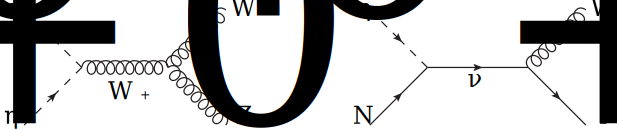
\includegraphics[scale=0.6]{coan}

efficient \hspace{4cm} suppressed by \alert{small} Yukawas couplings
  
\begin{align*}
 \sigma_\text{eff}^{N_i}\sim \sigma_\text{eff}\left(\frac{g_\text{eff}^0(x_\text{f.o.})}{g_\text{eff}^{N_i}(x_\text{f.o.})}\right)^2\qquad \text{$\sigma_\text{eff}^{N_i}$ decrease $\to$ $\Omega_{\text{DM}}$ increase} 
\end{align*}

\end{frame}

%%%%%%%%%%%%%%%%%%%%%%%

\begin{frame}\frametitle{Radiative type-I seesaw}
\begin{textblock*}{297mm}(60mm,0.5mm)%
\begin{beamercolorbox}[sep=0.01em,wd=6cm,center,rounded=true,shadow=true]{cite}
\scriptsize Klansen, D.R, Yaguna, Ruiz, Zapata, arXiv:1302.5298 (JCAP) 
\end{beamercolorbox}
\end{textblock*}
\begin{picture}(320,250)
\only<1>{\put(0,10){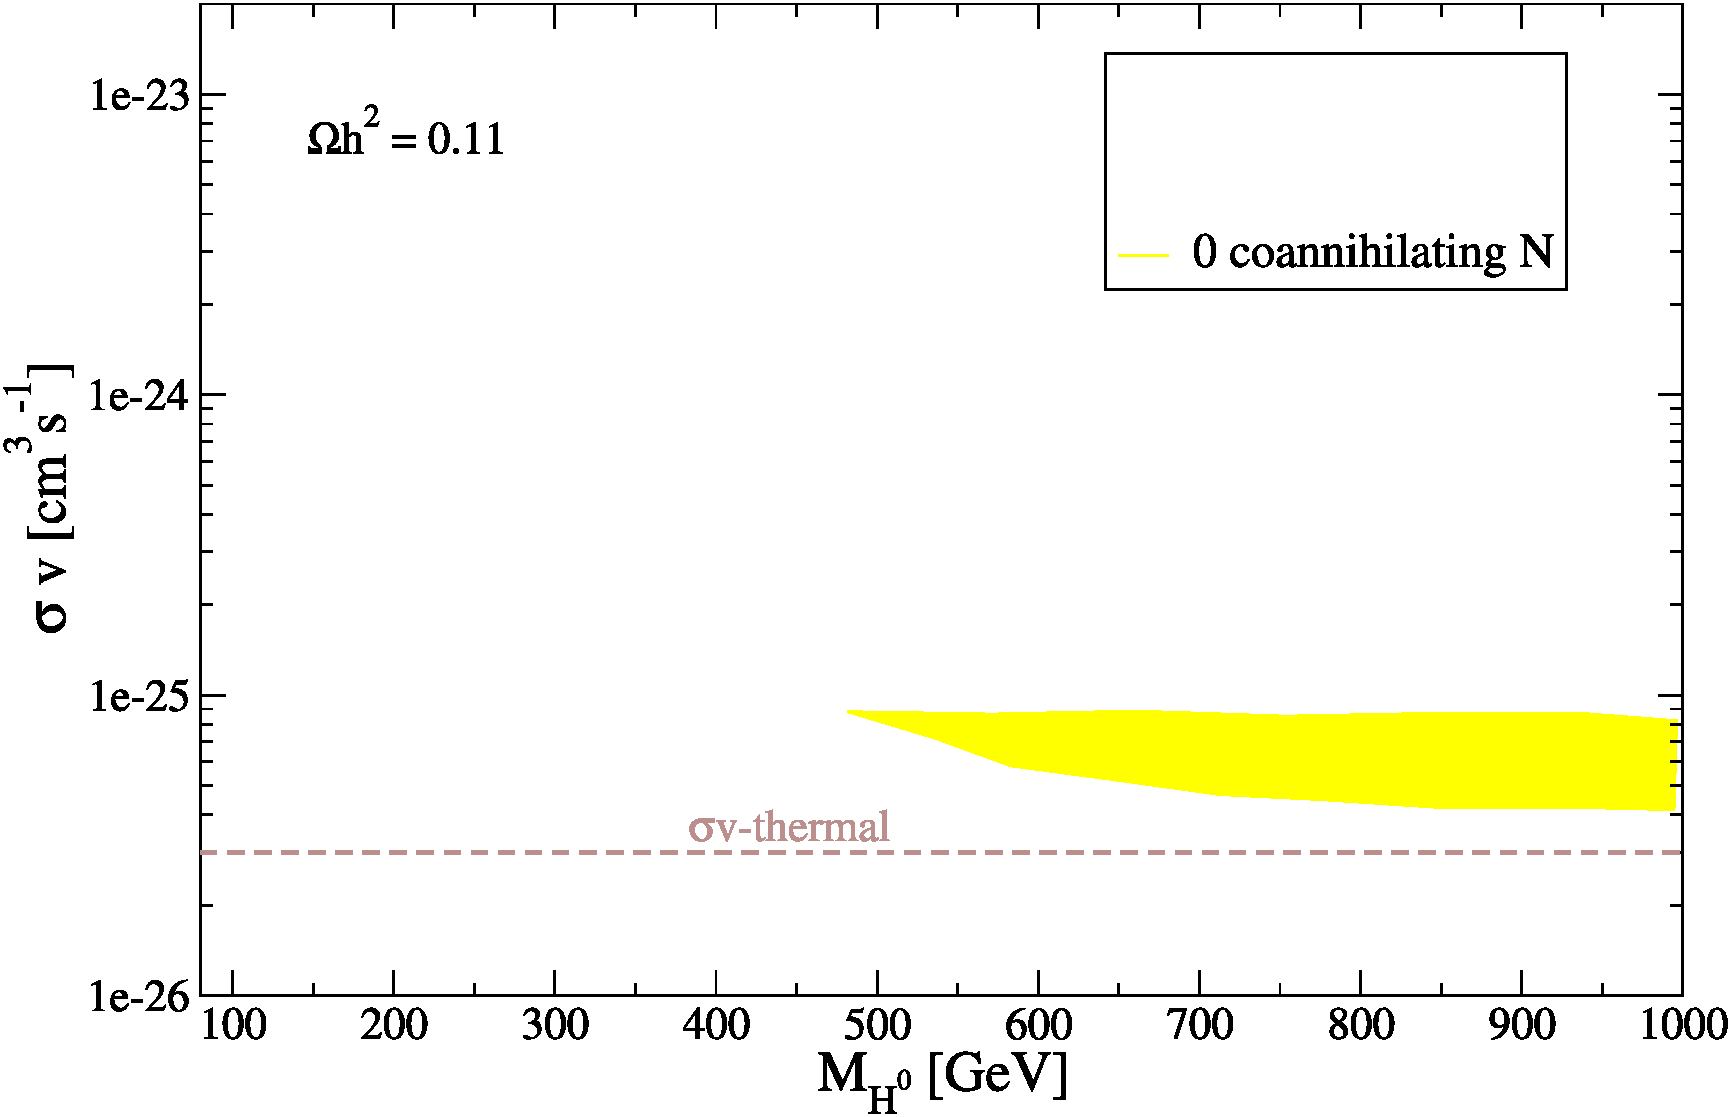
\includegraphics[scale=0.4]{sigmavdegB0}}}%
\only<2>{\put(0,10){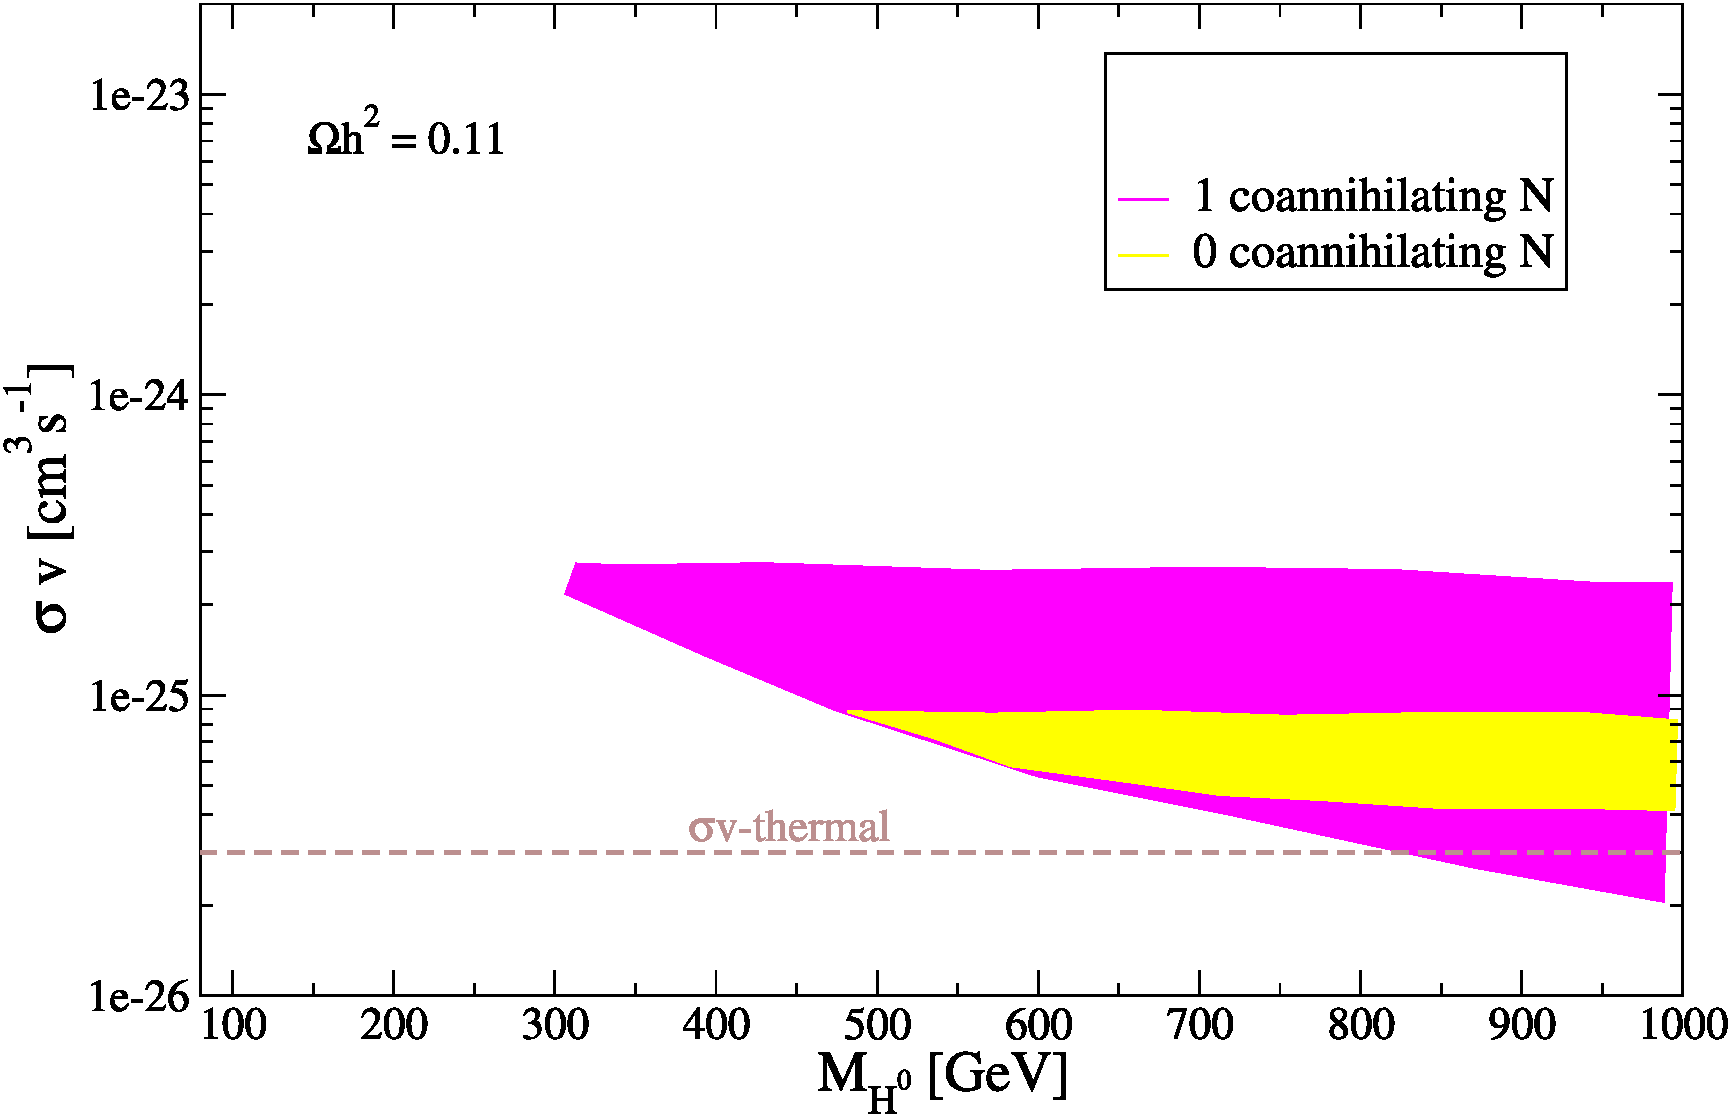
\includegraphics[scale=0.4]{sigmavdegB1}}}%
\only<3>{\put(0,10){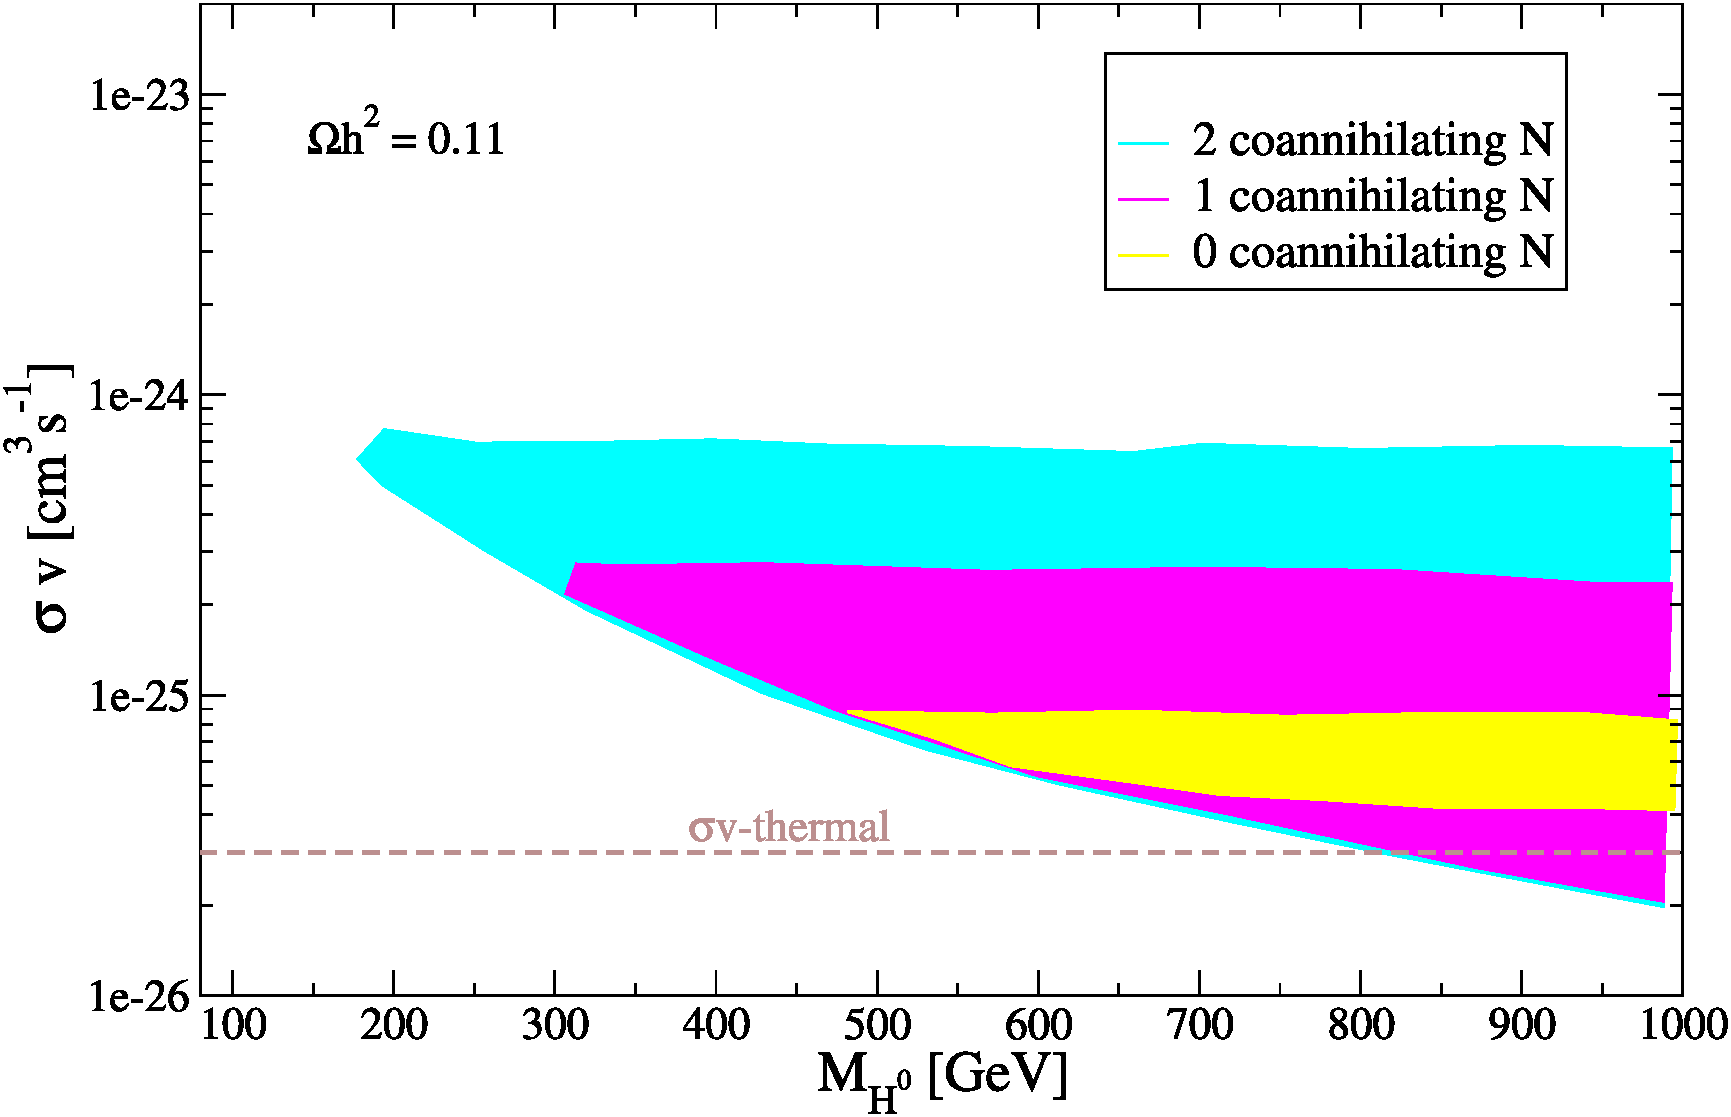
\includegraphics[scale=0.4]{sigmavdegB2}}}%
\only<4>{\put(0,10){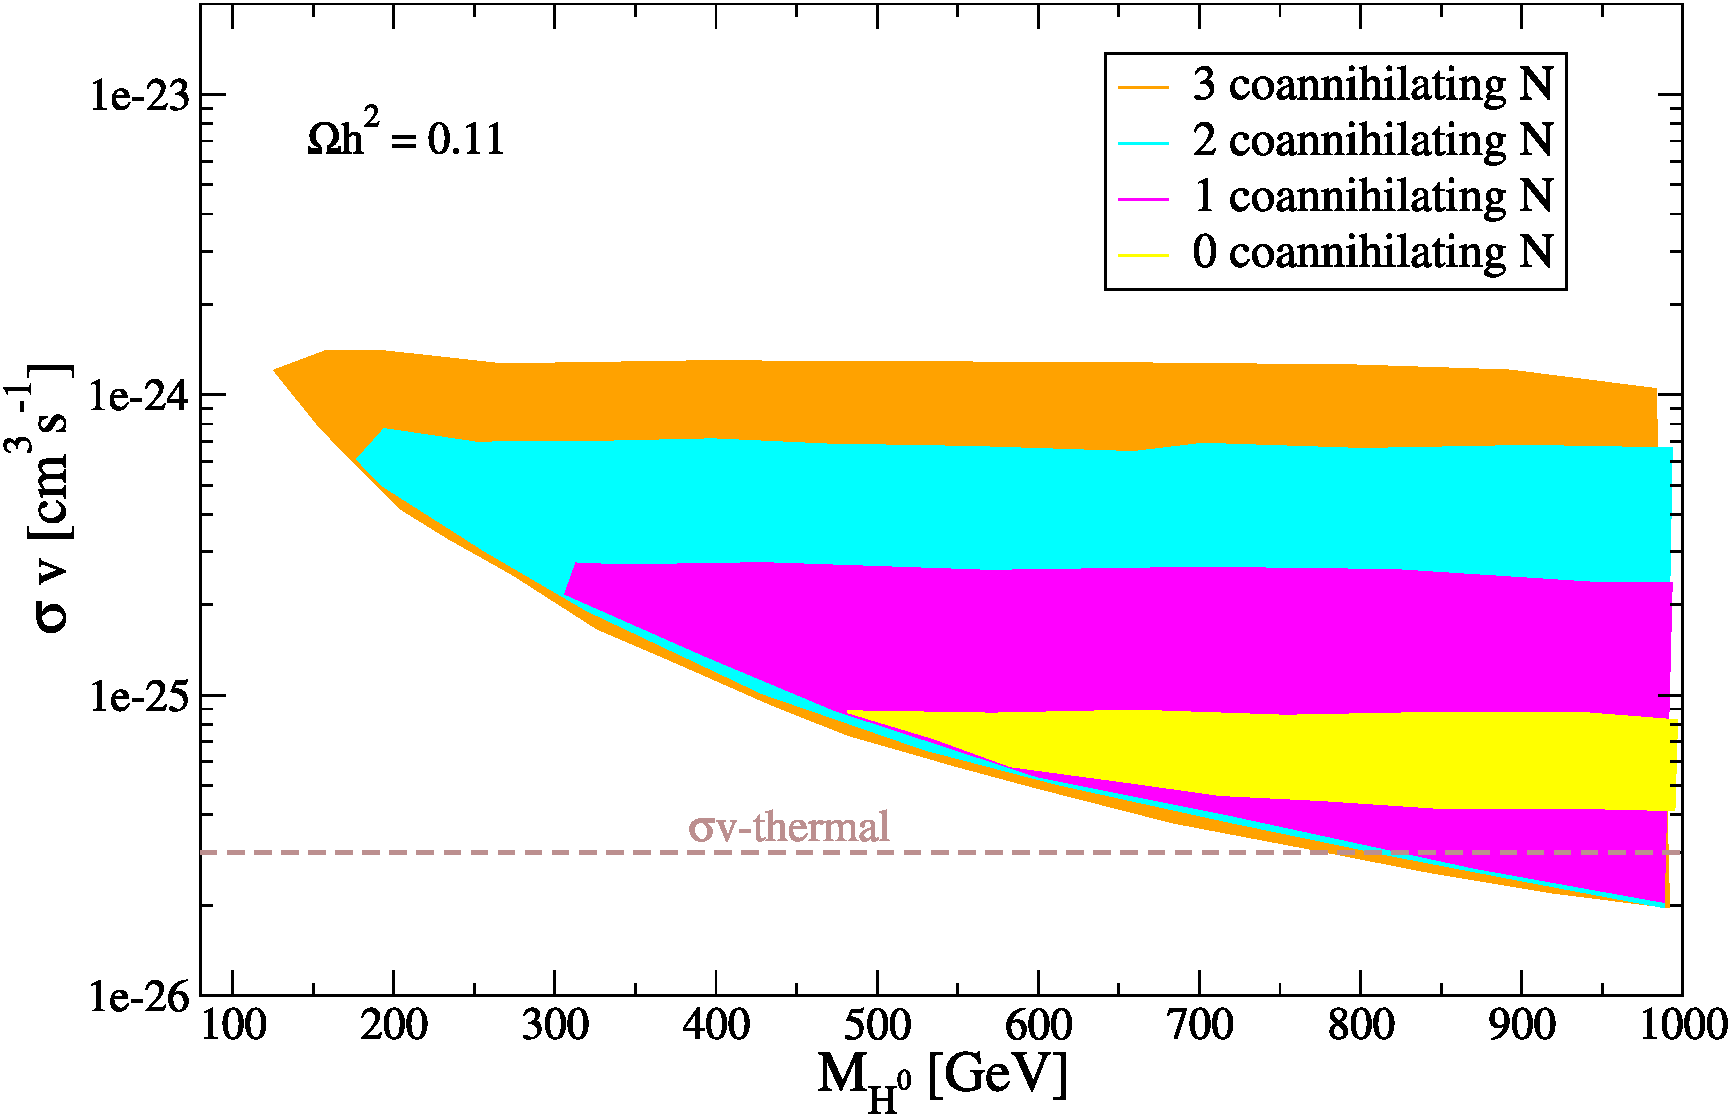
\includegraphics[scale=0.4]{sigmavdegB3}}}%
\only<5>{\put(0,10){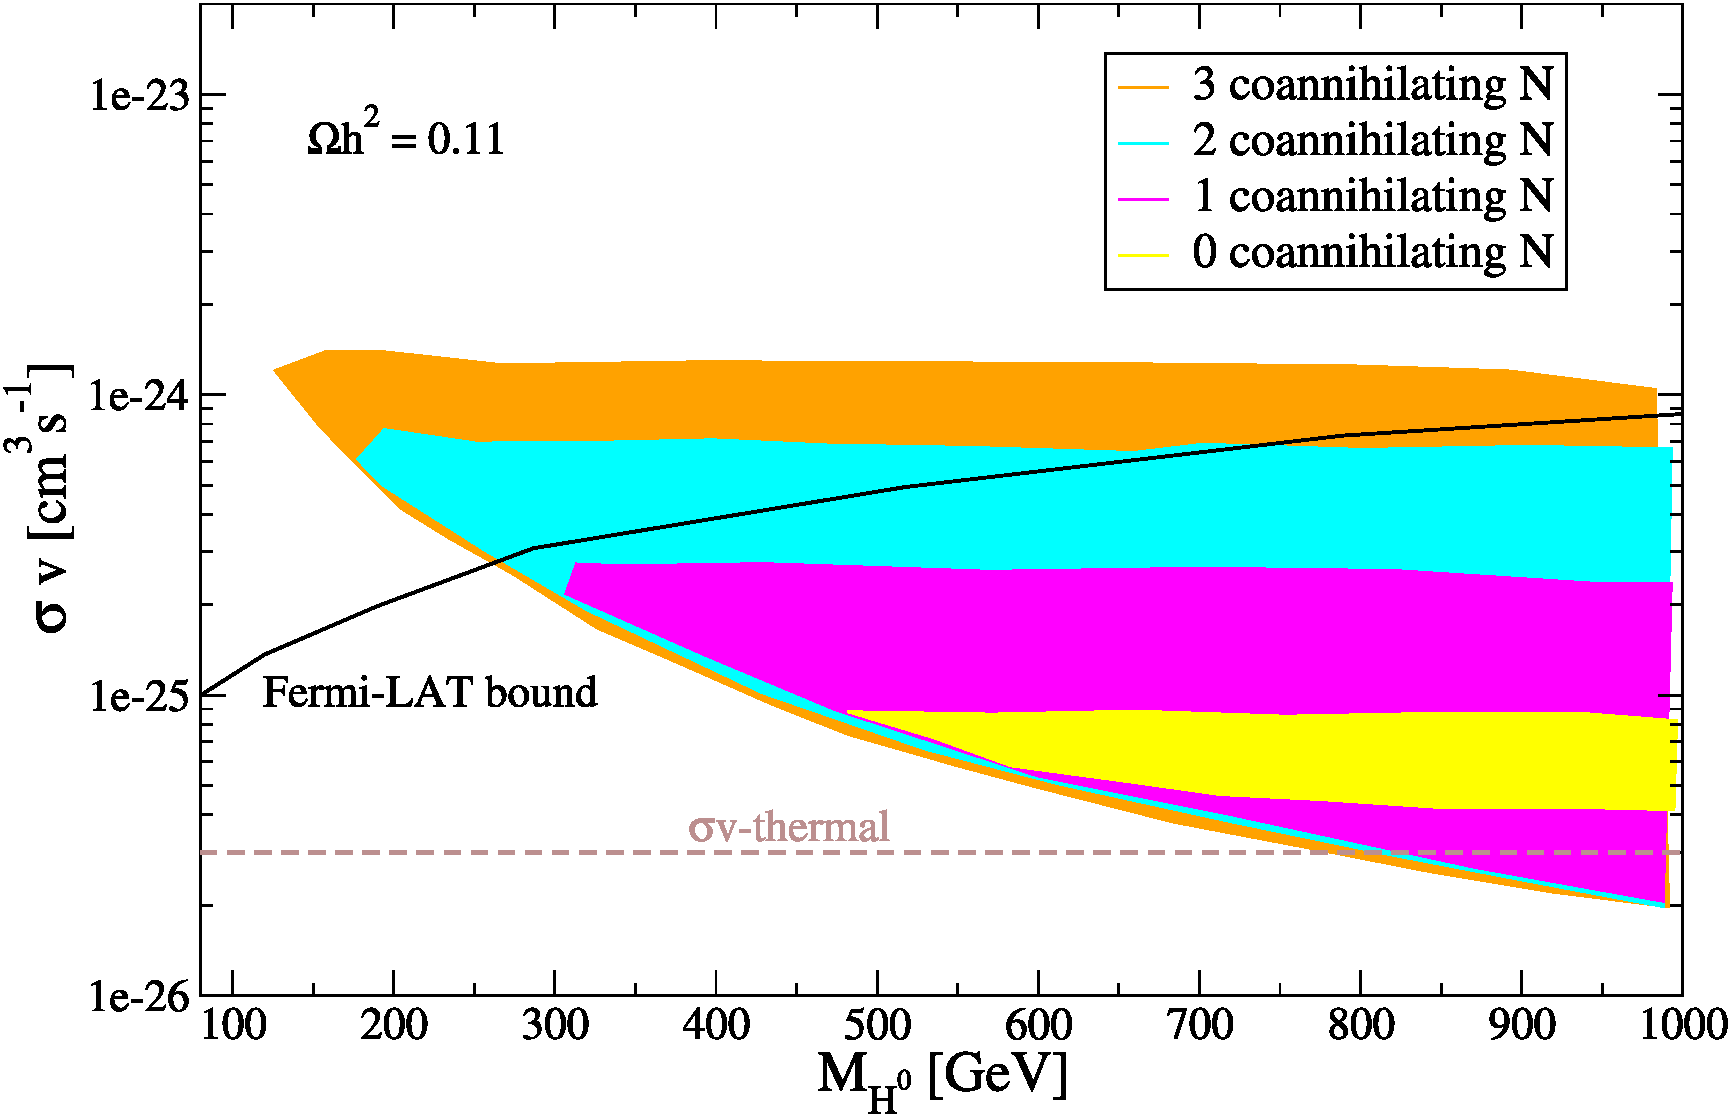
\includegraphics[scale=0.4]{sigmavdegB3F}}}%
\only<6->{\put(0,10){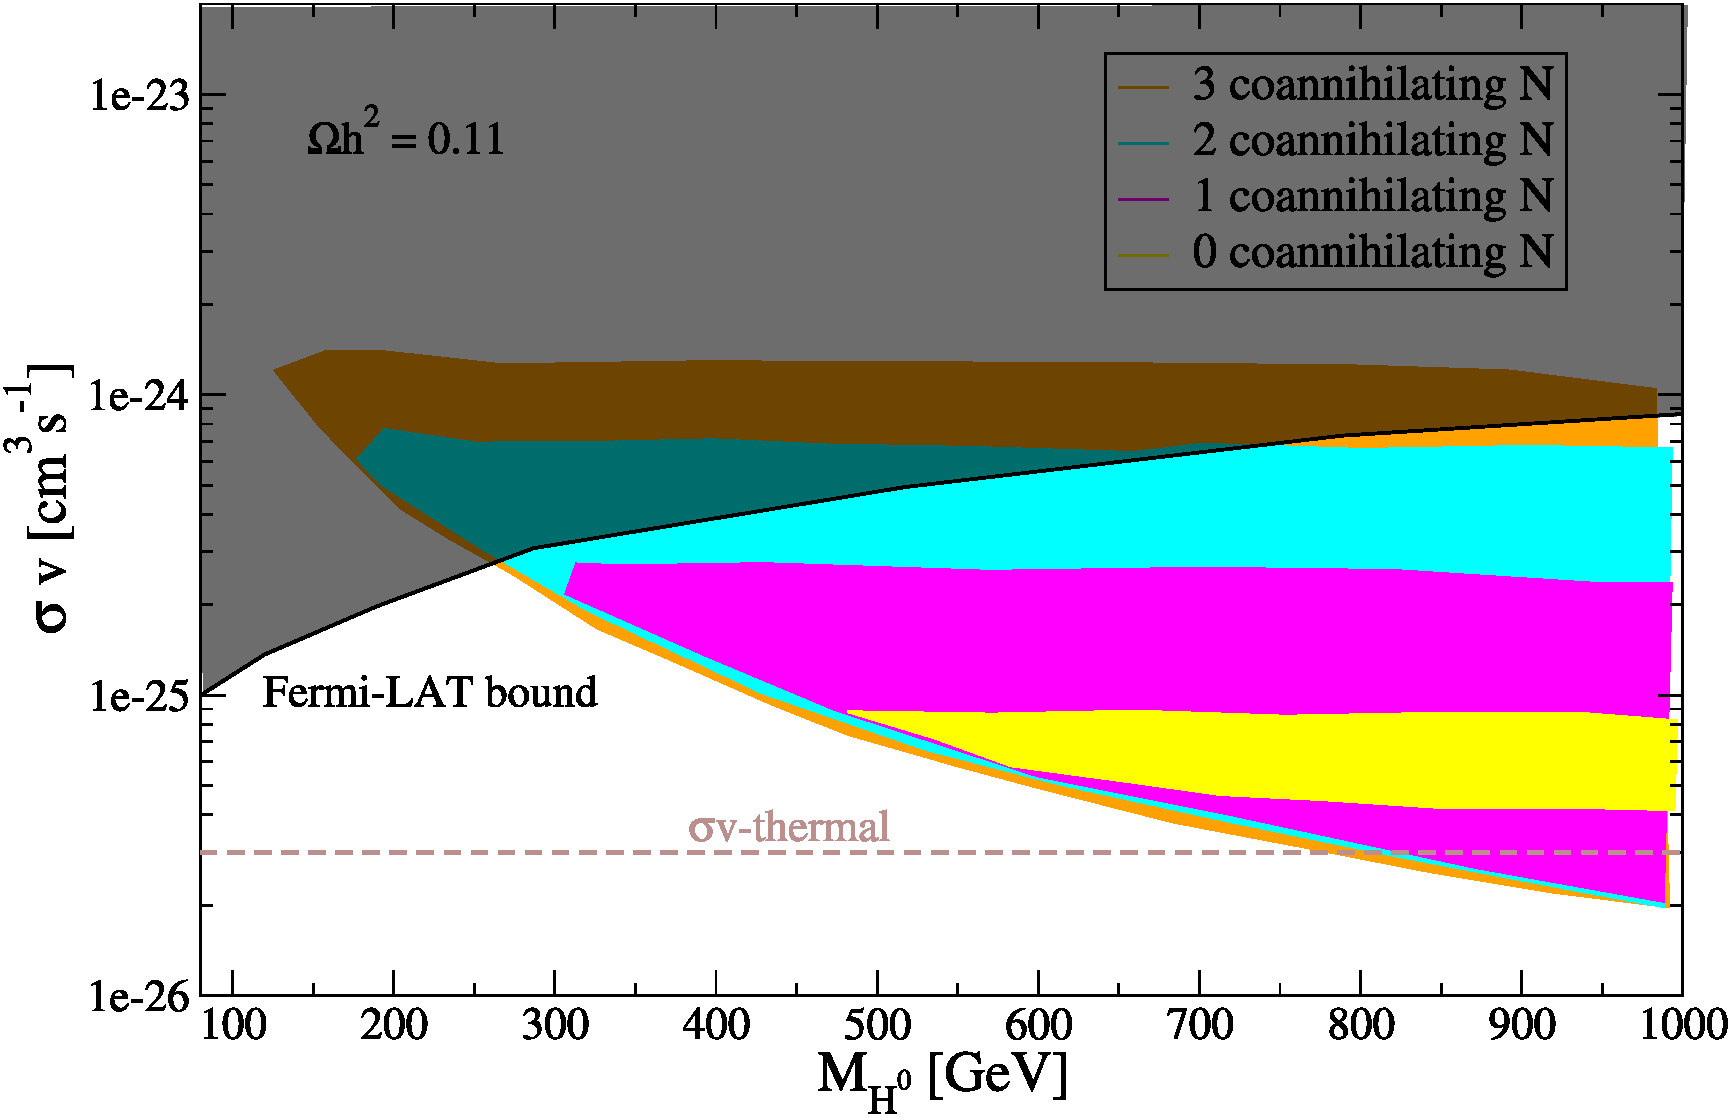
\includegraphics[scale=0.4]{sigmavdegB3FF}}}%
\only<6>{\put(10,225){\fcolorbox{black}{blue}{\color{white}%
\parbox[t]{10cm}{%
$N_i$ coannihilations allow to reconcile a thermal freeze-out 
with large values of $\left\langle \sigma v \right\rangle$
$\Longrightarrow$
Enhanced indirect detection signals
}}}}%
\only<7>{\put(10,225){\fcolorbox{black}{blue}{\color{white}%
\parbox[t]{10cm}{%
See also	
FIMP realization of the scotogenic model\\ 
Emiliano Molinaro, Carlos E. Yaguna, Oscar Zapata.\\
arXiv:1405.1259
}}}}%
\end{picture}  
\end{frame}
%%%%%%%

\begin{frame}[allowframebreaks]
  \frametitle{Tree level possibilities: }

\begin{textblock*}{297mm}(60mm,0.5mm)%
\begin{beamercolorbox}[sep=0.01em,wd=6cm,center,rounded=true,shadow=true]{cite}
\scriptsize Akhmedov, hep-ph/0001264; Langacker, arXiv:1112.5992
\end{beamercolorbox}
\end{textblock*}
%With the definition
%\begin{align*}
%  \psi^c=&C\bar{\psi}^T &\psi^c_L=&C\overline{\psi_L}^T\,.
%\end{align*}

The Majorana mass term should be  of the form $\overline{\nu^{c}_L}\nu_L$. Since
$\nu_L$ has $I_3=1/2$, the Majorana mass term
has $I_3=1$
%\footnote{Any $SU(2)$ spinor $\chi$, $\chi^T i\tau_2$ satisfy that
  % \begin{itemize}
  % \item both $\chi_1^{\dagger}\chi_2$ and $\chi_1^T i\tau \chi_2$ are invariant.
  % \item both $\chi_1^{\dagger}\boldsymbol{\tau}\chi_2$ and $\chi_1^T
  %   i\tau \boldsymbol{\tau}\chi_2$ transform as vectors.
  % \end{itemize}
%}. 
With $L=\begin{pmatrix}\nu_L&e_L\end{pmatrix}^T$
\begin{align*}
\overline{L^c}\boldsymbol{\tau}i\tau_2L&\sim \left( 3,-2 \right)\,.
\end{align*}
One would need an isotriplet scalar field $\Delta\sim (3,2)$, which
either elemental or composite. The term
\begin{align*}
  H^T \boldsymbol{\tau} i\tau_2H&\sim \left( 3,-2 \right),
\end{align*}
can play the role of the composite triplet, where $H=\begin{pmatrix}
H^+ & H^0\end{pmatrix}^T$

\end{frame}
%%%%%%%%%%%%%%

\begin{comentar}
  \begin{frame}[allowframebreaks]
Explicitly we have
\begin{align*}
  \overline{L^c}\boldsymbol{\tau}i\tau_2L=
  &\begin{pmatrix}
    \overline{\nu^c_L} & \overline{e^c_L}
  \end{pmatrix}\left[ 
  \begin{pmatrix}
    0 &1\\
    1 & 0\\    
  \end{pmatrix},
  \begin{pmatrix}
    0 &-i\\
    i & 0\\    
  \end{pmatrix},
  \begin{pmatrix}
    1 &0\\
    0 & -1\\    
  \end{pmatrix}
 \right]
 \begin{pmatrix}
   e_L\\
  -\nu_L\\
 \end{pmatrix}\nonumber\\
 =&\begin{pmatrix}
    \overline{\nu^c_L} & \overline{e^c_L}
  \end{pmatrix}\left[ 
  \begin{pmatrix}
    -\nu_L\\
    e_L\\
  \end{pmatrix},
  i\begin{pmatrix}
    \nu_L\\
    e_L\\
  \end{pmatrix},
  \begin{pmatrix}
    e_L\\
    \nu_L\\
  \end{pmatrix}
 \right]\nonumber\\
  =&\left(\overline{e^c_L}e_L-\overline{\nu^c_L}\nu_L,
    i\left(\overline{\nu^c_L}\nu_L+\overline{e^c_L}e_L\right),
   \overline{\nu^c_L}e_L+\overline{e^c_L}\nu_L
   \right)
\end{align*}
Replacing back $\overline{\nu^c_L}\to H^+$, $\overline{e^c_L}\to H^0$, $\nu_L\to H^+$, and $e_L\to H^0$, we have
\begin{align*}
H^T \boldsymbol{\tau} i\tau_2H=&
  \left(H^0H^0-H^+H^+,
    i\left( H^0H^0+H^+H^+ \right),
   H^+H^0+H^+H^+
   \right).
\end{align*}
\begin{align}
\label{eq:details}
&\left(\overline{L^c}\boldsymbol{\tau}i\tau_2L\right)\cdot
  \left( H^T \boldsymbol{\tau} i\tau_2H\right)\nonumber\\
&=2 \left( 
-\overline{e^c_L}e_LH^+H^+-\overline{\nu^c_L}\nu_LH^0H^0
 +\overline{\nu^c_L}e_LH^+H^0
+\overline{e^c_L}\nu_LH^+H^0\right)\nonumber\\
&=-2\left( \overline{\nu^c_L}H^0-\overline{e^c_L}H^+ \right)
\left( H^0\nu_L-H^+e_L \right)\\
&=-2\left[
  \begin{pmatrix}
    \overline{\nu^c_L}& \overline{e^c_L}
  \end{pmatrix}
  \begin{pmatrix}  
    H^0\\
   -H^+    
  \end{pmatrix}
\right]\left[ 
  \begin{pmatrix}
    H^0 & -H^+
  \end{pmatrix}
  \begin{pmatrix}
   \nu_L\\
   e_L\\    
  \end{pmatrix}
 \right]\nonumber
\end{align}
\end{frame}
\end{comentar}
%%%%%%%
\begin{frame}
  We have the Weinberg operator
  \begin{align*}
    \mathcal{L}=&  -\frac{f}{2M}\left(\overline{L^c}\boldsymbol{\tau}i\tau_2L\right)\cdot
  \left( H^T \boldsymbol{\tau} i\tau_2H\right)+\text{h.c}\nonumber\\
=&\frac{f}{M}\left( \overline{L^c}\widetilde{H}^{*} \right)
\left( \widetilde{H}^{\dagger}L \right)+\text{h.c}\nonumber\\
=&\frac{f}{M}\overline{L^c_a}H_cL_bH_d\epsilon_{ac}\epsilon_{bd}+\text{h.c}\,.
\text{\hspace{1cm}\begin{beamercolorbox}[sep=0.01em,wd=4cm,center,rounded=true,shadow=true]{cite}
\scriptsize Weinberg,  PRL43(1979)1566
\end{beamercolorbox}
}
\end{align*}




\end{frame}
%%%%%%%
{
\setbeamertemplate{background}{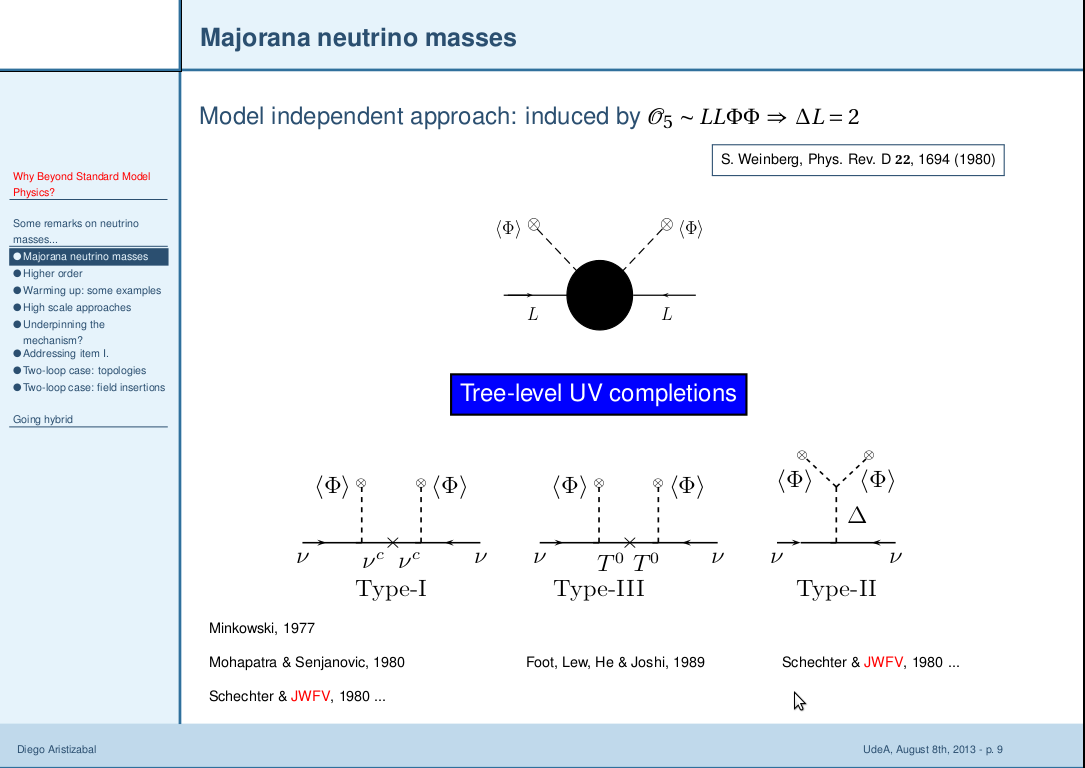
\includegraphics[width=\paperwidth]{daristi}}
\begin{frame}[plain]

\begin{picture}(320,250)
\only<1->{\put(150,-5){\begin{beamercolorbox}[sep=0.01em,wd=6cm,center,rounded=true,shadow=true]{cite}
Diego Aristizabal \MVAt\ FestiValle (2013)
\end{beamercolorbox}
}}%
\only<2>{\put(0,22){\begin{beamercolorbox}[sep=0.01em,wd=12cm,center,rounded=true,shadow=true]{white}
Finite number of models with fixed hypercharges and representations 

(Even with $\left\langle \Phi \right\rangle\to \left\langle S_{1,2} \right\rangle$ \begin{beamercolorbox}[sep=0.01em,wd=5.7cm,center,rounded=true,shadow=true]{cite}
\scriptsize McDonald, arXiv:1303.4573 (JHEP)
\end{beamercolorbox}\quad)
\end{beamercolorbox}
}}%
\only<3>{\put(130,123){\fcolorbox{black}{blue}{\color{white}One-loop UV completions}%
}}%
\only<3>{\put(55,25){\begin{beamercolorbox}[sep=2.3em,wd=10cm,center,rounded=true,shadow=true]{white}
Arbitrary  number of models:

Multiple hypercharges and representations.
\end{beamercolorbox}
}}%
\end{picture}
\end{frame}
}
%%%%%%%%%%%%%%%%%%%%%%%%
\begin{frame}
  \frametitle{Weinberg operator at one-loop}
\begin{textblock*}{297mm}(68mm,0.5mm)%
\begin{beamercolorbox}[sep=0.01em,wd=5.7cm,center,rounded=true,shadow=true]{cite}
\scriptsize Bonnet, Hirsch, Ota, Winter, arXiv:1204.5862 (JHEP)
\end{beamercolorbox}
\end{textblock*}

  \begin{block}{Notations}
    \begin{center}
      \begin{align*}
        \alert{\mathbf{X}}^{\color{OliveGreen}\mathcal{L}}_{\color{blue}\mathbf{Y}}
      \end{align*}
      \begin{itemize}
      \item $\color{OliveGreen}\mathcal{L}$ Lorentz nature: scalar ($\color{OliveGreen}S$) or fermion ($\color{OliveGreen}F$),
      \item $\color{blue}Y\equiv 2(Q-I_3)$ hypercharge: $\color{blue}\alpha$ arbitrary rational-number
      \item $\alert{\mathbf{X}}$ $SU(2)$ nature: singlet $\alert{\mathbf{1}}$, doublet $\alert{\mathbf{2}}$, triplet $\alert{\mathbf{3}}$
        \begin{itemize}
        \item quadruplet $\alert{\mathbf{4}}$, quintuplet $\alert{\mathbf{5}}$, $\ldots$ \begin{beamercolorbox}[sep=0.01em,wd=5.7cm,center,rounded=true,shadow=true]{cite}
\scriptsize Law, McDonald, arXiv:1305.6467
\end{beamercolorbox}

        \end{itemize}

      \end{itemize}
    \end{center}
  \end{block}
\end{frame}
%%%%%%%%%%%%%%%%%%%%%%%%%%%%%%
\begin{frame}
\frametitle{Weinberg operator at one-loop}
\only<1>{\begin{textblock*}{297mm}(68mm,0.5mm)%
\begin{beamercolorbox}[sep=0.01em,wd=5.7cm,center,rounded=true,shadow=true]{cite}
\scriptsize Ma, hep-ph/9805219 (PRL)
\end{beamercolorbox}
\end{textblock*}
}%  
\only<2->{\begin{textblock*}{297mm}(68mm,0.5mm)%
\begin{beamercolorbox}[sep=0.01em,wd=5.7cm,center,rounded=true,shadow=true]{cite}
\scriptsize Bonnet, Hirsch, Ota, Winter, arXiv:1204.5862 (JHEP)
\end{beamercolorbox}
\end{textblock*}
}%  
\begin{picture}(320,250)
\only<2->{\put(0,140){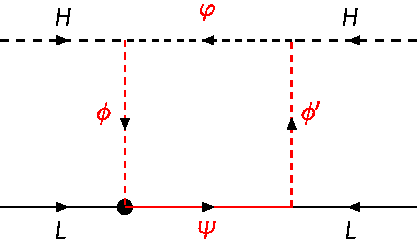
\includegraphics[scale=0.8]{T1-1}}}%
\only<1->{\put(180,140){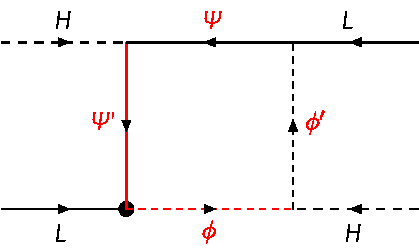
\includegraphics[scale=0.8]{T1-2}}}%
\only<1->{\put(0,20){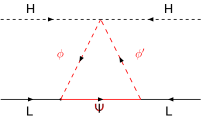
\includegraphics[scale=0.8]{T3}}}%
\only<1->{\put(180,20){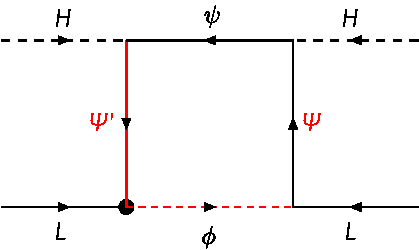
\includegraphics[scale=0.8]{T1-3}}}%
\only<2>{\put(170,5){and reducible and divergent topologies}}%
\only<3->{\put(40,110){\fcolorbox{black}{blue}{\color{white}Radiative seesaw}
}}%
\only<3->{\put(80,25){\color{red}\circle{12}}}%
\only<3->{\put(0,6){\fbox{$\alert{1}^{F}_{\color{blue}1+\alpha}\,,
\alert{2}^{F}_{\color{blue}1+\alpha}\,,
\alert{3}^{F}_{\color{blue}1+\alpha}\,,
\alert{4}^{F}_{\color{blue}1+\alpha}\,,
\alert{5}^{F}_{\color{blue}1+\alpha}\,,\cdots$}}}%
\only<4->{\put(233,186){\fcolorbox{black}{blue}{\color{white}Zee model}
}}%
\end{picture}
\end{frame}
%%%%%%%%%%%%%%%%%%%%%%%%%%%%%%

\begin{frame}\frametitle{Generalized Zee model}
\begin{picture}(320,250)
%%%REFERENCES
\only<1>{\put(150,250){\begin{beamercolorbox}[sep=0.01em,wd=6cm,center,rounded=true,shadow=true]{cite}
\scriptsize A. Zee, Phys.Lett.B93(1980)389 .
\end{beamercolorbox}%
}}%
\only<2>{\put(150,250){\begin{beamercolorbox}[sep=0.01em,wd=6cm,center,rounded=true,shadow=true]{cite}
\scriptsize E. Ma, hep-ph/9805219 (PRL)
\end{beamercolorbox}%
}}%
\only<3>{\put(150,250){\begin{beamercolorbox}[sep=0.01em,wd=6cm,center,rounded=true,shadow=true]{cite}
\scriptsize Bonnet, Hirsch, Ota, Winter, arXiv:1204.5862 (JHEP)
\end{beamercolorbox}%
}}%
\only<4>{\put(150,250){\begin{beamercolorbox}[sep=0.01em,wd=6cm,center,rounded=true,shadow=true]{cite}
\scriptsize [?]
\end{beamercolorbox}%
}}%
\only<5->{\put(150,250){\begin{beamercolorbox}[sep=0.01em,wd=6cm,center,rounded=true,shadow=true]{cite}
\scriptsize D.R, Yagunga, Zapata,  arXiv:1308.3655
\end{beamercolorbox}%
}}%

\only<1->{\put(2,160){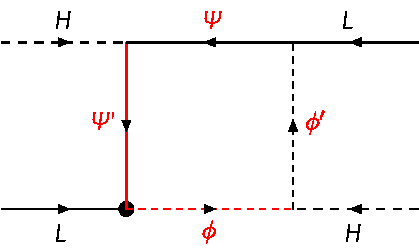
\includegraphics[scale=0.7]{T1-2}%
}}
\put(145,120){\renewcommand{\arraystretch}{1.3}
\rowcolors{1}{RoyalBlue!20}{RoyalBlue!5}
  \begin{tabular}{p{1.1cm}|p{1.1cm}|p{1.1cm}|p{1.1cm}|p{0.5cm}}
    $\psi$ & $\phi$ & $\phi'$ & $\psi'$&\only<5->{$\alpha$}\\
%row2
\only<3-4>{$\alert{1^F_\alpha}$}    \only<5->{$\alert{\mathbf{1}^F_0}$}    &%
\only<3-4>{$\alert{2^S_{1+\alpha}}$}\only<5->{$\alert{\mathbf{2}^S_{1}}$}&%
\only<3-4>{$\alert{1^S_\alpha}$}    \only<5->{$\alert{\mathbf{1}^S_0}$}    &%
\only<3-4>{$\alert{2^F_{1+\alpha}}$}\only<5->{$\alert{2^F_{1}}$}&%
\only<6>{\fbox{$0$}}\only<7->{$0$}\\
%row 4
\only<1>{$2^F_1\text{:}\;\overline{e_{L}}$}%
\only<2-4>{$\alert{2^F_\alpha}$}
\only<5->{$\alert{2^F_{-1}}$}&%
\only<1>{$1^S_2\text{:}\;\eta^+$}%
\only<2-4>{$\alert{1^S_{1+\alpha}}$}%
\only<5->{$\alert{1^S_{-2}}$}&%
\only<1>{$2^S_1\text{:}\;\phi$}%
\only<2-4>{$\alert{2^S_\alpha}$}%
\only<5->{$\alert{\mathbf{2}^S_{-1}}$}&%
\only<1>{$1^F_2\text{:}\;\overline{e_{R}}$}%
\only<2-4>{$\alert{1^F_{1+\alpha}}$}%
\only<5->{$\alert{1^F_{-2}}$}&%
\only<7>{\fbox{$-2$}}\only<8->{$-2$}\\ 
%row3
\only<3-4>{$\color{blue}1^F_\alpha$}%
\only<5->{$\color{blue}\mathbf{1}^F_0$}&%
\only<3-4>{$\color{blue}2^S_{1+\alpha}$}%
\only<5->{$\color{blue}\mathbf{2}^S_{1}$}&%
\only<3-4>{$\color{blue}3^S_\alpha$}%
\only<5->{$\color{blue}{3}^S_0$}&%
\only<3-4>{$\color{blue}2^F_{1+\alpha}$}%
\only<5->{$\color{blue}2^F_{1}$}&%
\only<6>{\fbox{$0$}}\only<7->{$0$}\\ 
%row6
\only<2-4>{$\color{blue}2^F_\alpha$}%
\only<5->{$\color{blue}2^F_{-1}$}&%
\only<2-4>{$\color{blue}3^S_{1+\alpha}$}%
\only<5->{$\color{blue}3^S_{-2}$}&%
\only<2-4>{$\color{blue}2^S_\alpha$}%
\only<5->{$\color{blue}\mathbf{2}^S_{-1}$}&%
\only<2-4>{$\color{blue}1^F_{1+\alpha}$}%
\only<5->{$\color{blue}1^F_{-2}$}&%
\only<7>{\fbox{$-2$}}\only<8->{\fbox{$\mathbf{-2}$}}\\ 
%row7
\only<2-4>{$\color{OliveGreen}2^F_\alpha$}%
\only<5->{$\color{OliveGreen}2^F_1$}&%
\only<2-4>{$\color{OliveGreen}3^S_{1+\alpha}$}%
\only<5->{$\color{OliveGreen}3^S_{2}$}&%
\only<2-4>{$\color{OliveGreen}2^S_\alpha$}%
\only<5->{$\color{OliveGreen}\mathbf{2}^S_1$}&%
\only<2-4>{$\color{OliveGreen}3^F_{1+\alpha}$}%
\only<5->{$\color{OliveGreen}3^F_{2}$}&%
\only<7>{\fbox{$1$}}\only<8->{\fbox{$\mathbf{1}$}}\\ 
%row9
\only<3-4>{$\color{OliveGreen}3^F_\alpha$}%
\only<5->{$\color{OliveGreen}\mathbf{3}^F_0$}&%
\only<3-4>{$\color{OliveGreen}2^S_{1+\alpha}$}%
\only<5->{$\color{OliveGreen}\mathbf{2}^S_{-1}$}&%
\only<3-4>{$\color{OliveGreen}3^S_\alpha$}%
\only<5->{$\color{OliveGreen}\mathbf{3}^S_0$}&%
\only<3-4>{$\color{OliveGreen}2^F_{1+\alpha}$}%
\only<5->{$\color{OliveGreen}2^F_{-1}$}&%
\only<6>{\fbox{$-1$}}\only<7->{$-1$}\\  
%row 5
\only<2-4>{$2^F_\alpha$}%
\only<5->{$2^F_1$}&%
\only<2-4>{$1^S_{1+\alpha}$}%
\only<5->{$1^S_{2}$}&%
\only<2-4>{$2^S_\alpha$}%
\only<5->{$\mathbf{2}^S_1$}&%
\only<2-4>{$3^F_{1+\alpha}$}%
\only<5->{$3^F_{2}$}&%
\only<7>{\fbox{$1$}}\only<8->{\fbox{$\mathbf{1}$}}\\ 
%row8
\only<3-4>{$3^F_\alpha$}%
\only<5->{$\mathbf{3}^F_0$}&%
\only<3-4>{$2^S_{1+\alpha}$}%
\only<5->{$\mathbf{2}^S_{-1}$}&%
\only<3-4>{$1^S_\alpha$}%
\only<5->{$\mathbf{1}^S_0$}&%
\only<3-4>{$2^F_{1+\alpha}$}%
\only<5->{$2^F_{-1}$}&%
\only<6>{\fbox{$-1$}}\only<7->{$-1$}\\ 
\multicolumn{4}{c}{\only<4->{Larger $SU(2)_L$ multiplets}}&%
\\
  \end{tabular}%
}%
\only<3>{\put(20,80){\huge$\alert{\alpha\to-\alpha-1}$}}%
\only<5>{\put(-20,170){\parbox[t]{6cm}{
      \begin{center}
        \textbf{Dark matter filter}
      \end{center}
\vspace{-0.5cm}

      \begin{itemize}
      \item Impose $Z_2$ symmetry
        \begin{itemize}
        \item SM particles are even
        \item New particles are odd
        \end{itemize}
      \item Lightest odd particle (LOP)
        \begin{itemize}
        \item Color and electrically neutral
        \item Consistent with direct detection constraints
        \end{itemize}
      \item Odd fermions must be vector-like
      \end{itemize}
}}}%
\only<5>{\put(10,10){\fcolorbox{black}{blue}{\color{white}$Y=-2T_3$ for at least one particle}%
}}%
\only<6>{\put(0,100){\begin{beamercolorbox}[sep=0.1em,wd=4.7cm,center,rounded=true,shadow=true]{white}
\alert{Radiative type-I/III seesaw } with
additional contribution to neutrino masses.
\end{beamercolorbox}
}}%
\only<6>{\put(2,10){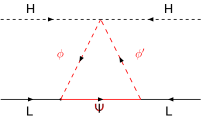
\includegraphics[scale=0.7]{T3}}
}%
\only<7-8>{\put(0,100){\begin{beamercolorbox}[sep=0.1em,wd=4.7cm,center,rounded=true,shadow=true]{white}
\alert{Inert doublet model} with
 one-loop neutrino masses (susy-like)
\end{beamercolorbox}
}}%
\only<8>{\put(0,60){\begin{beamercolorbox}[sep=0.1em,wd=4.7cm,center,rounded=true,shadow=true]{white}
and exotic charges
\end{beamercolorbox}
}}

\end{picture}  
\end{frame}
%%%%%%%
%%%%%%%%%%%%%%%%%%%%%%%%
\begin{frame}[plain]
\begin{picture}(320,250)
\only<1>{\put(-12,-13){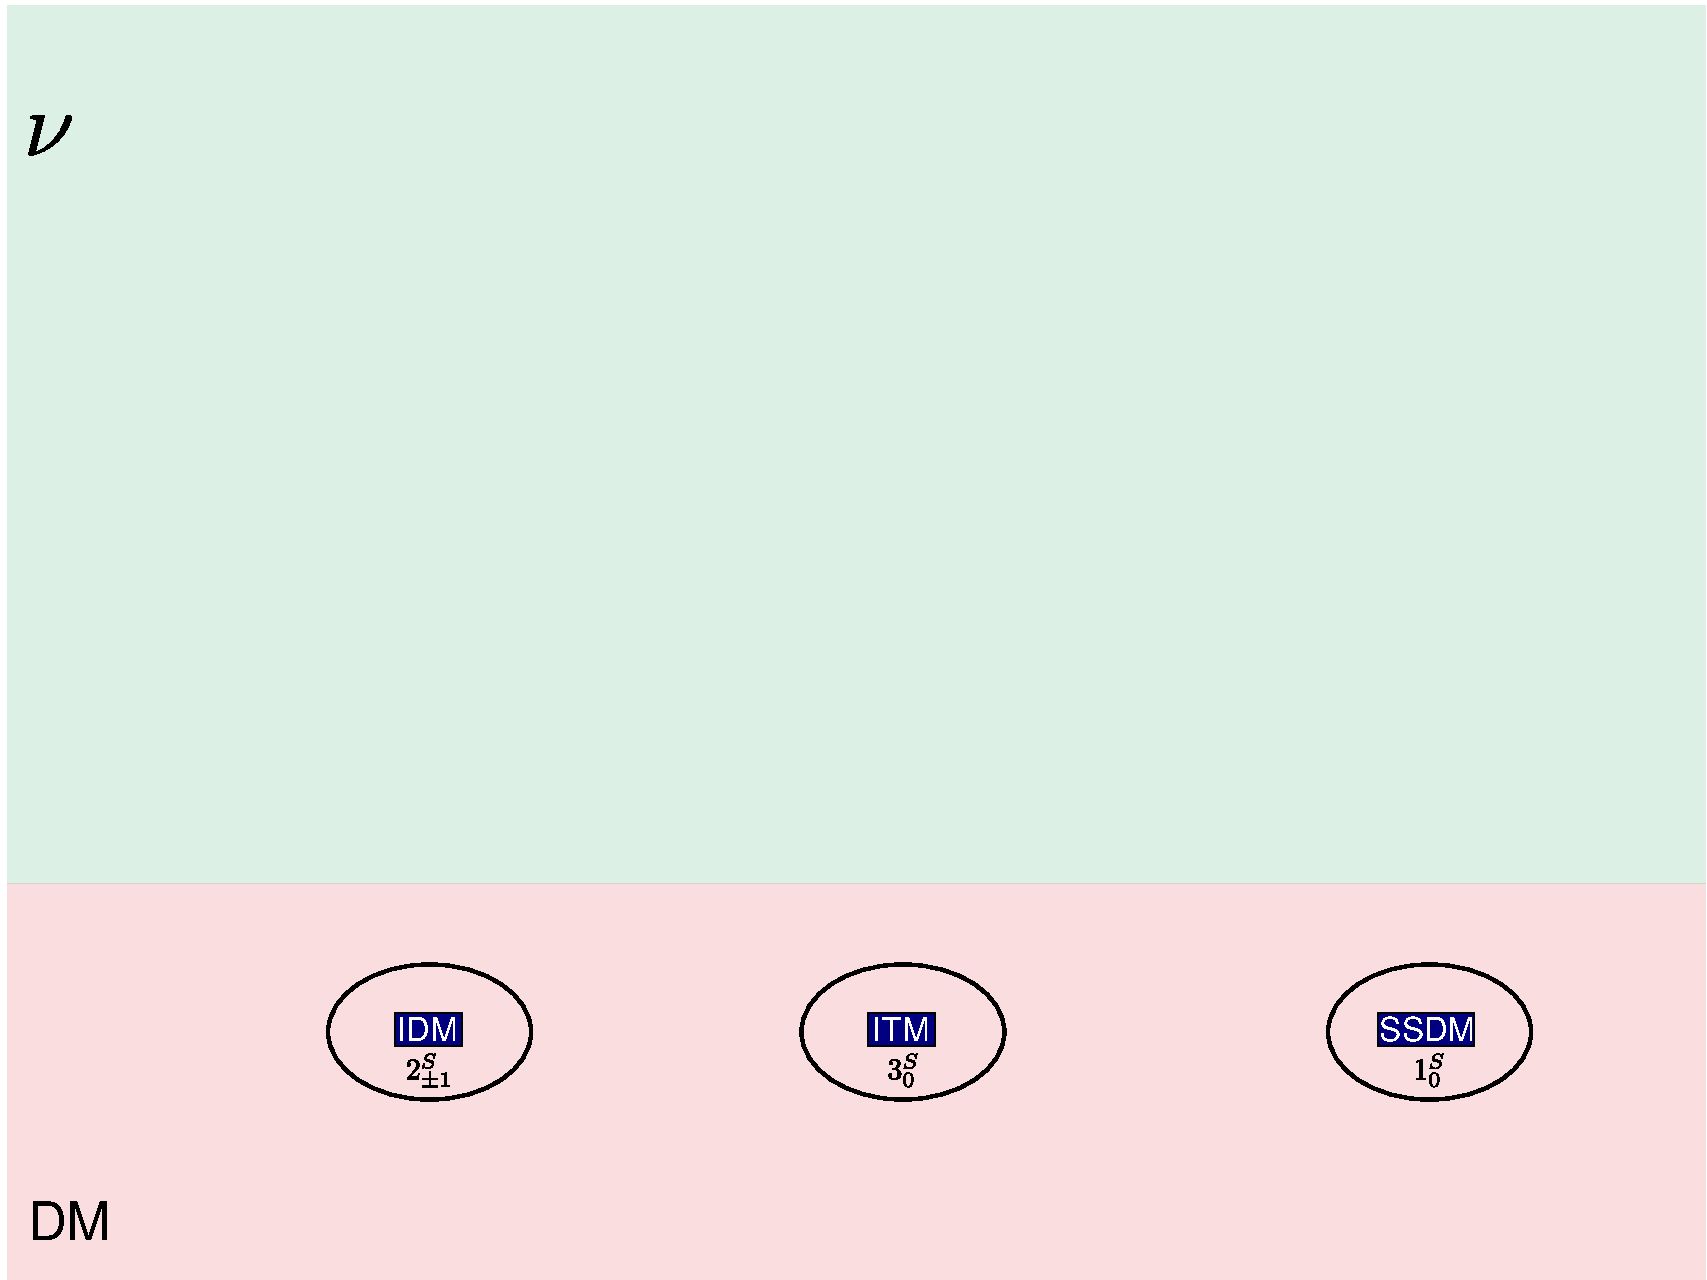
\includegraphics[width=\paperwidth,height=\paperheight]{dmwmodels1}}}%
\only<2>{\put(-12,-13){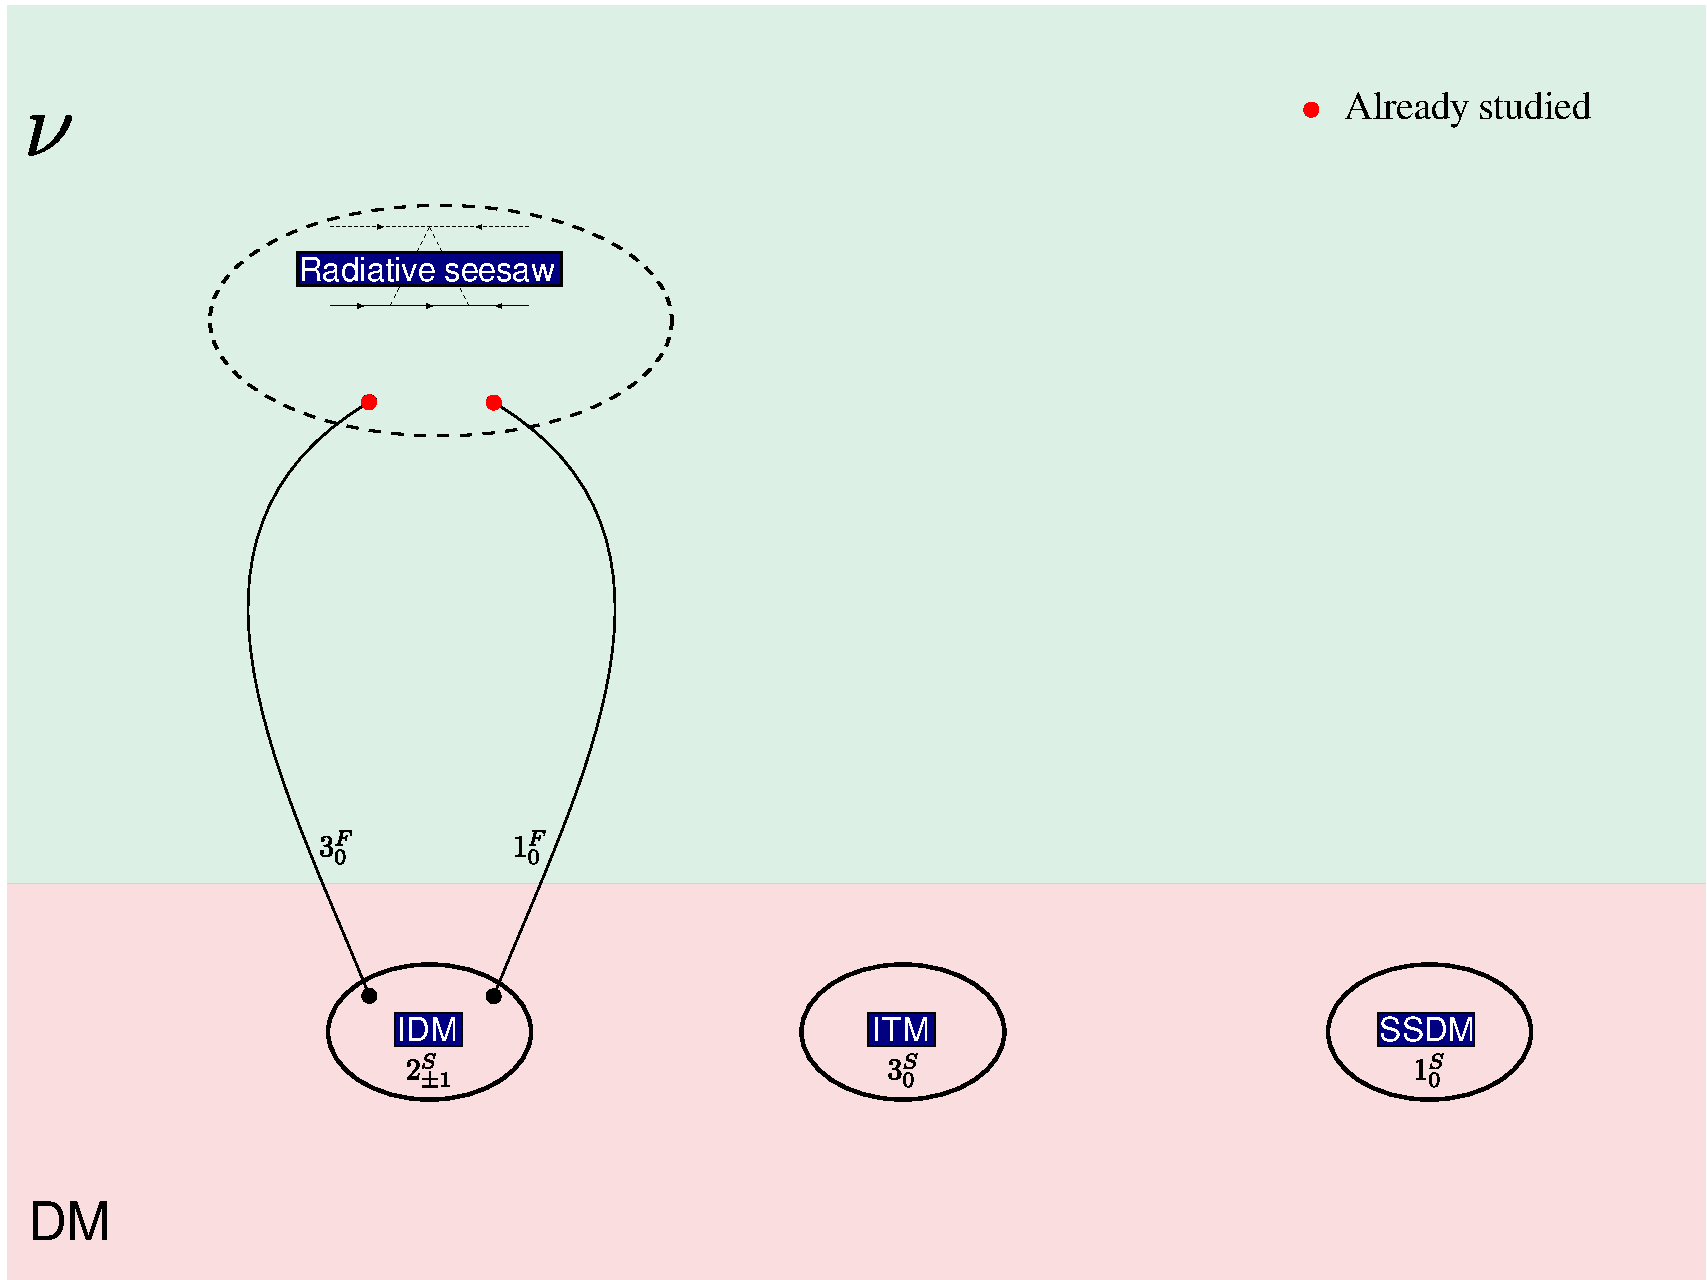
\includegraphics[width=\paperwidth,height=\paperheight]{dmwmodels2}}}%
\only<3>{\put(-12,-13){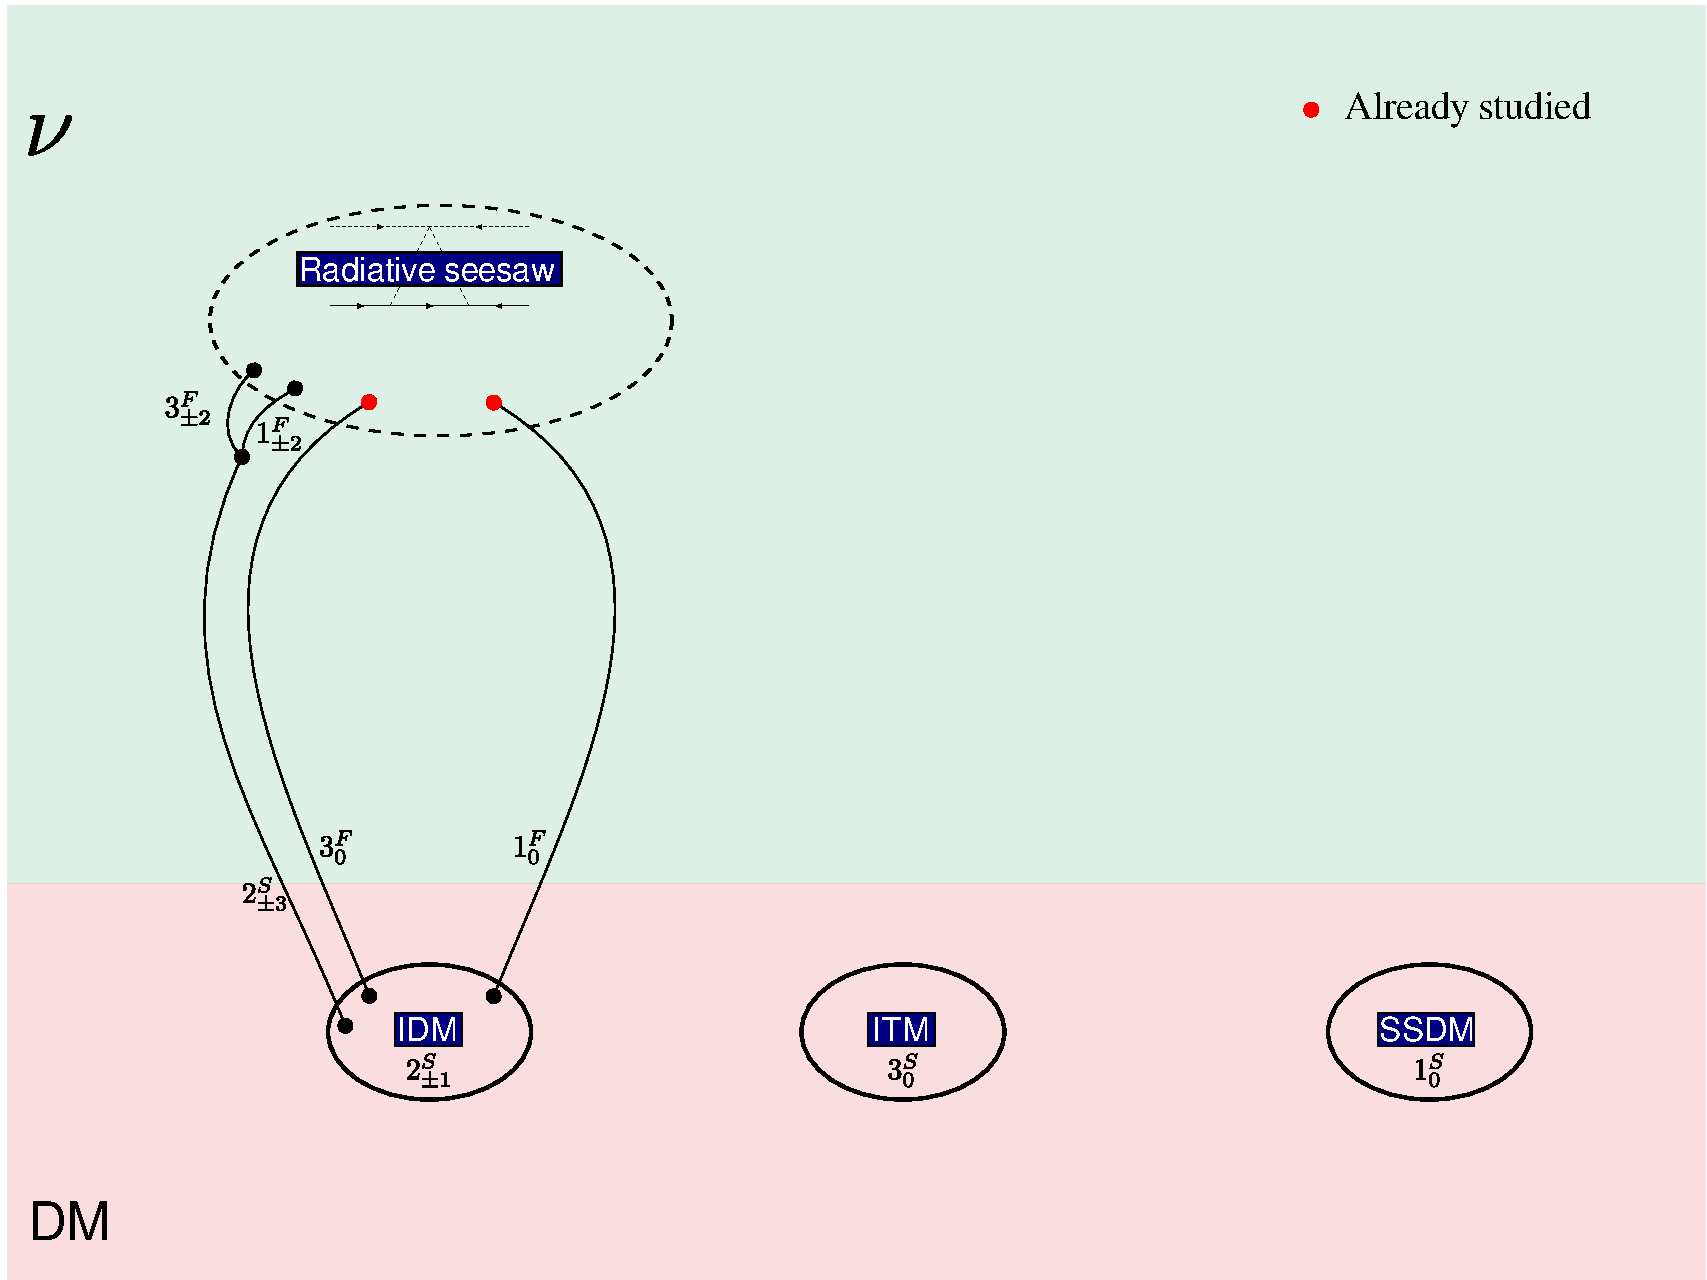
\includegraphics[width=\paperwidth,height=\paperheight]{dmwmodels3}}}%
\only<4>{\put(-12,-13){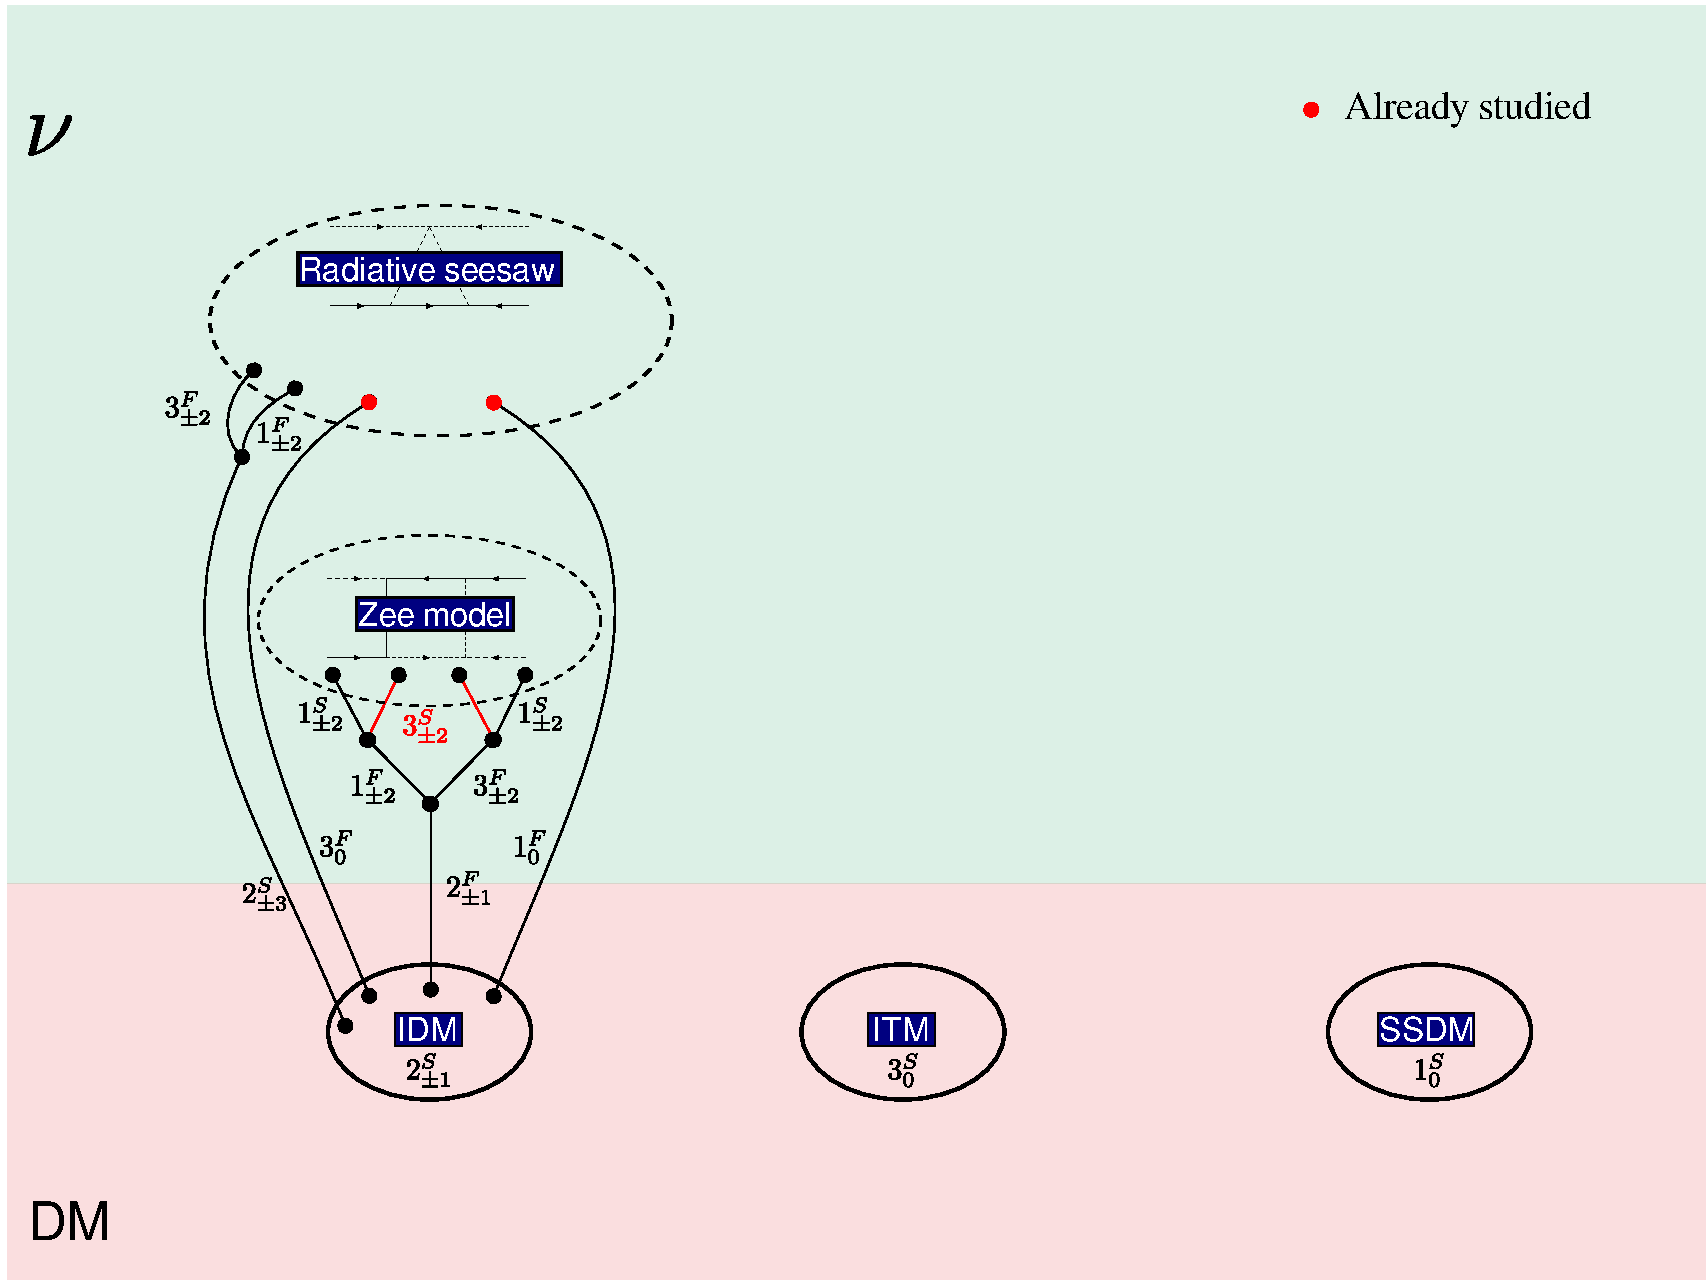
\includegraphics[width=\paperwidth,height=\paperheight]{dmwmodels4}}}%
\only<5>{\put(-12,-13){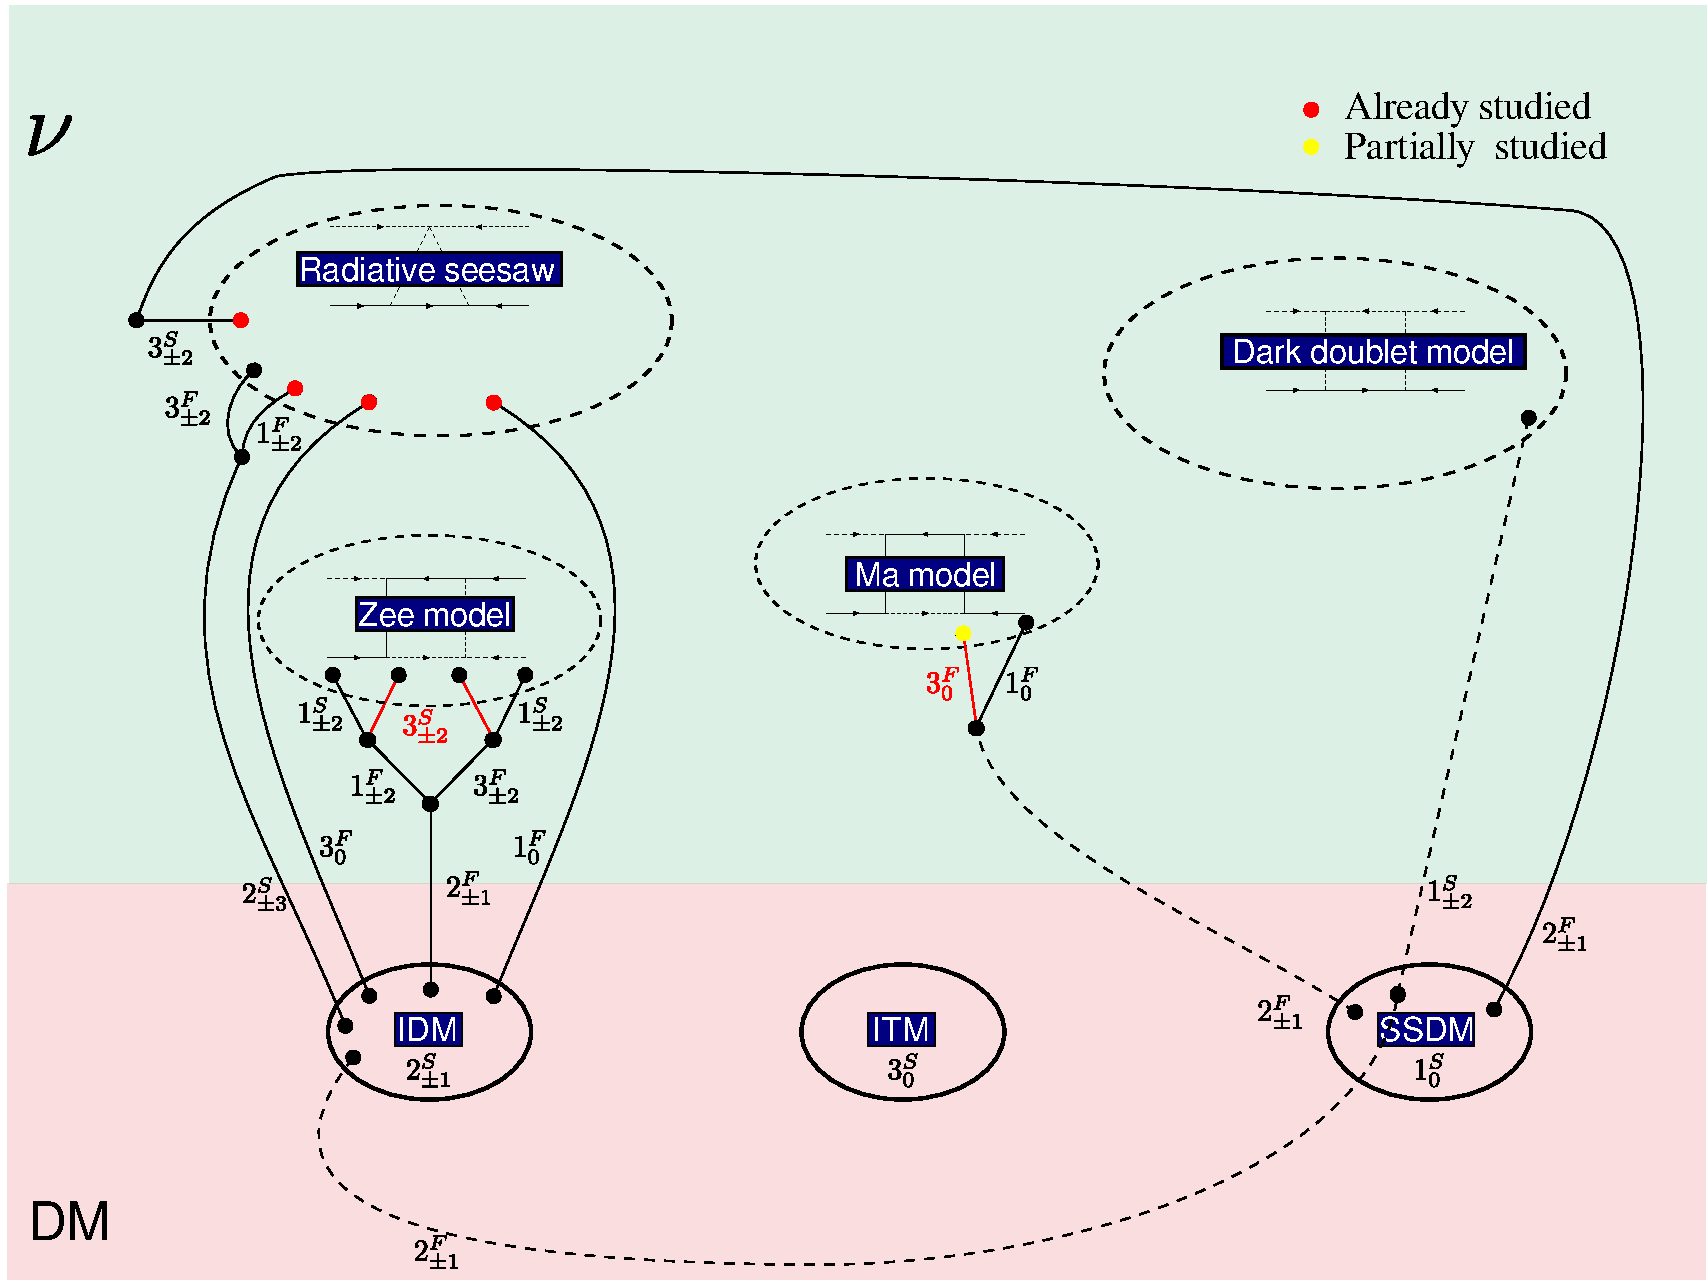
\includegraphics[width=\paperwidth,height=\paperheight]{dmwmodels5}}}%
\only<6>{\put(-12,-13){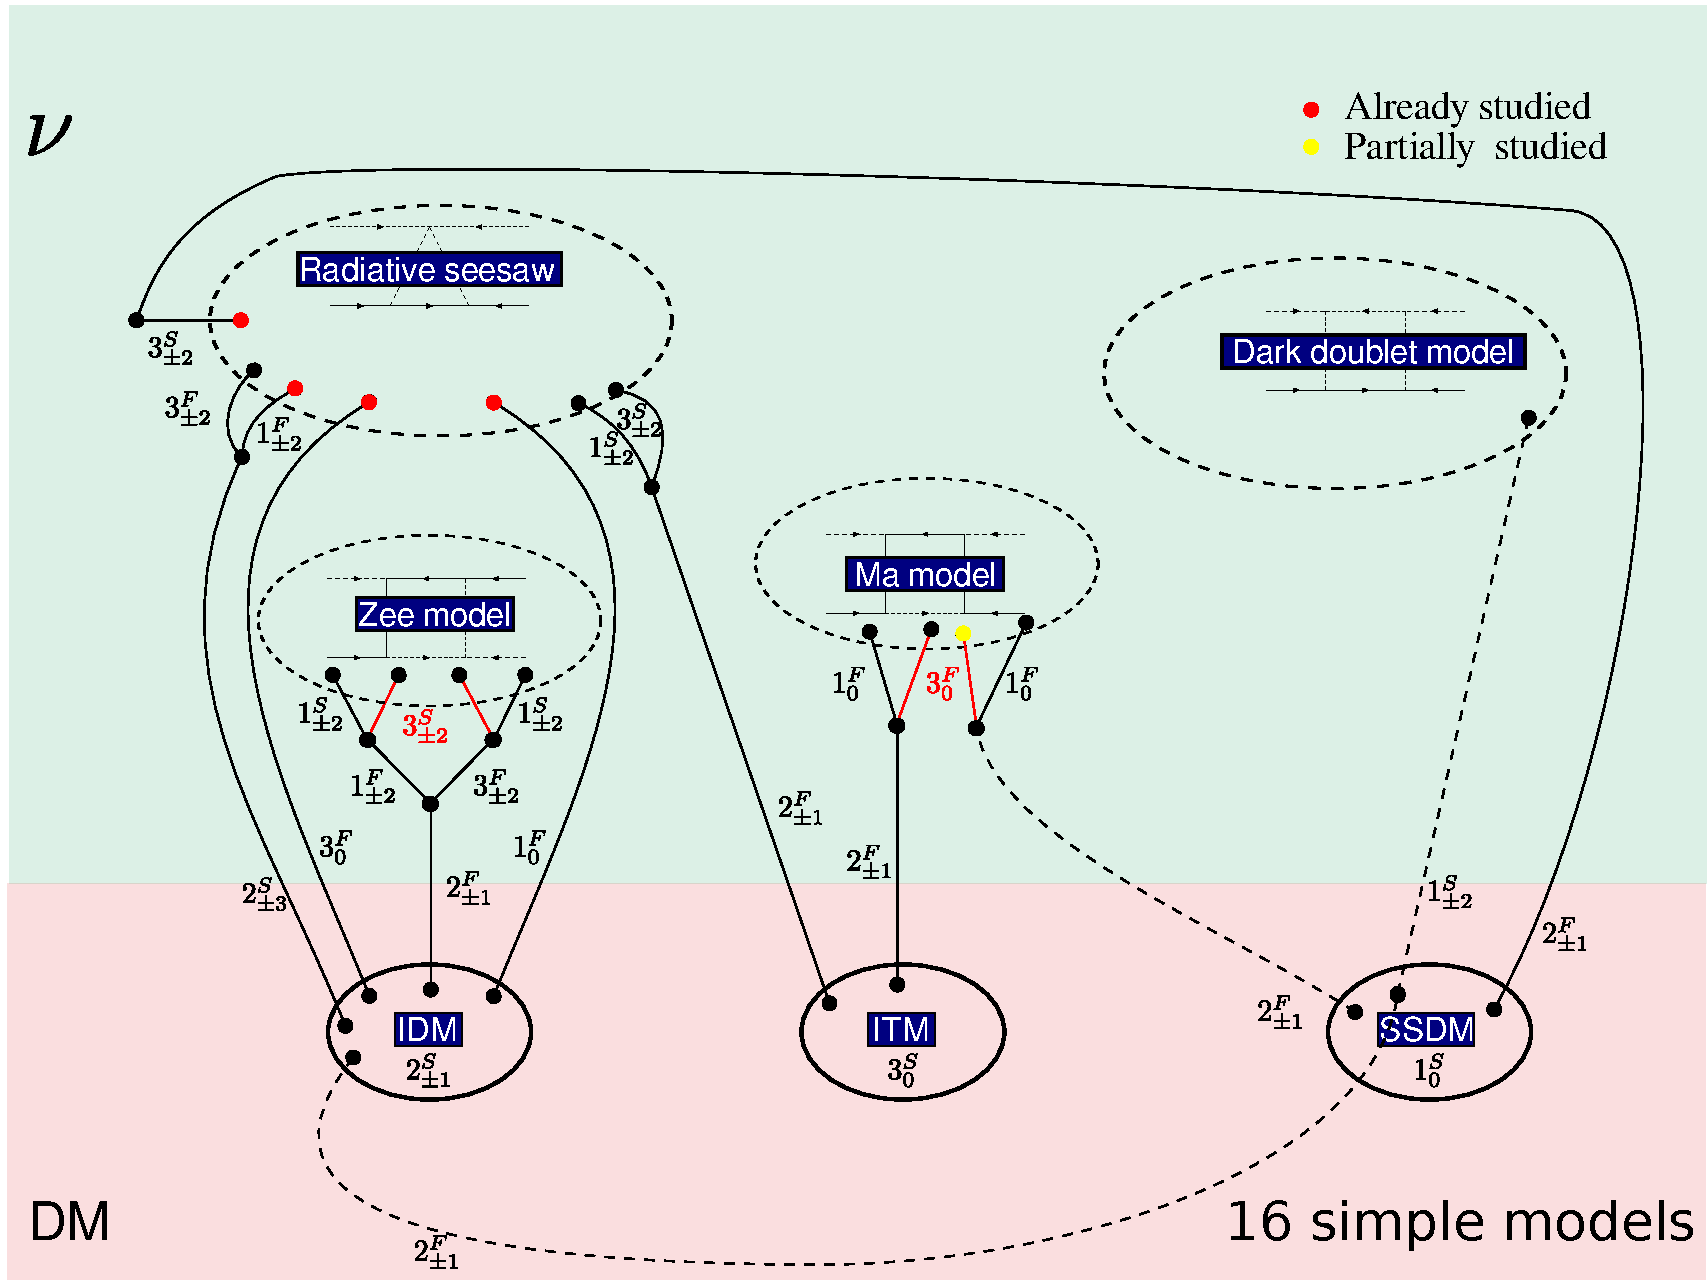
\includegraphics[width=\paperwidth,height=\paperheight]{dmwmodels6}}}%
\only<7>{\put(-12,-13){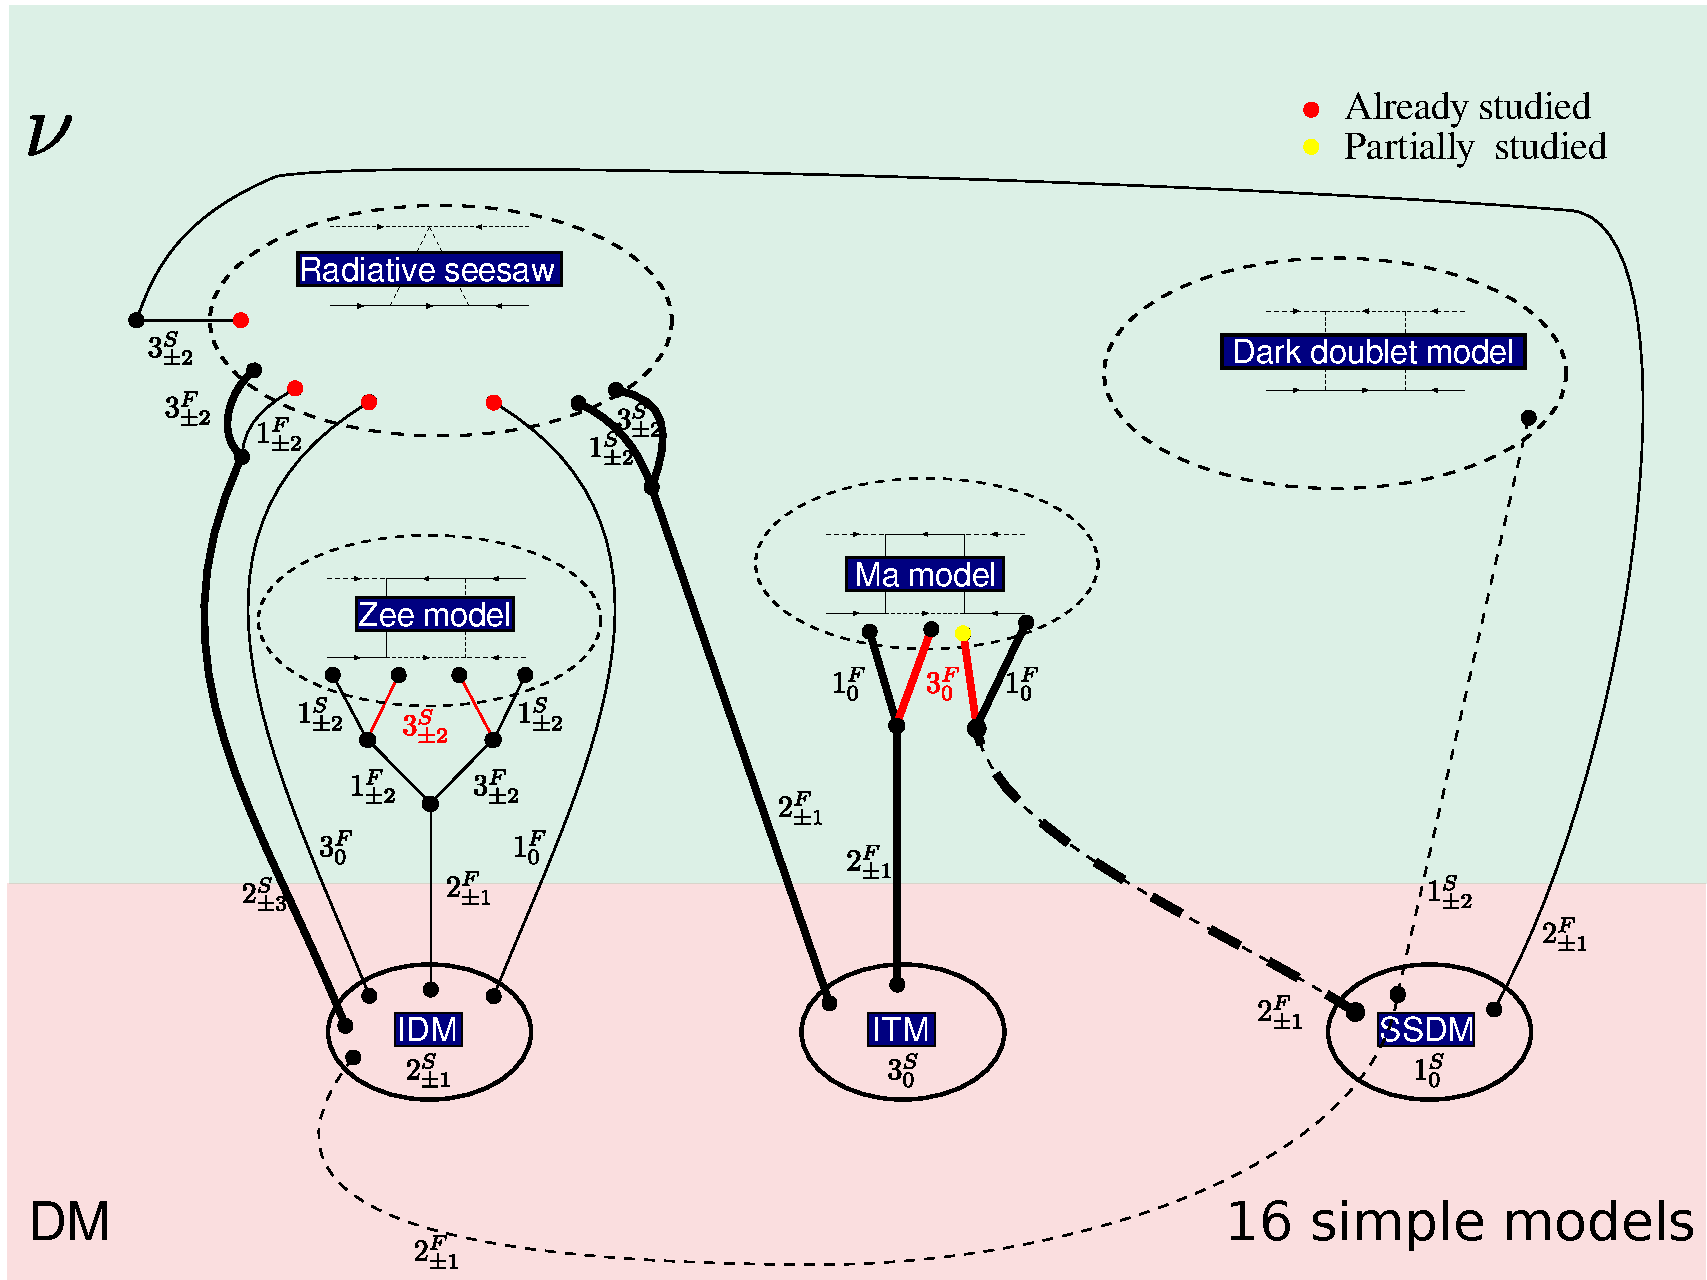
\includegraphics[width=\paperwidth,height=\paperheight]{dmwmodels7}}}%
\only<8>{\put(-12,-13){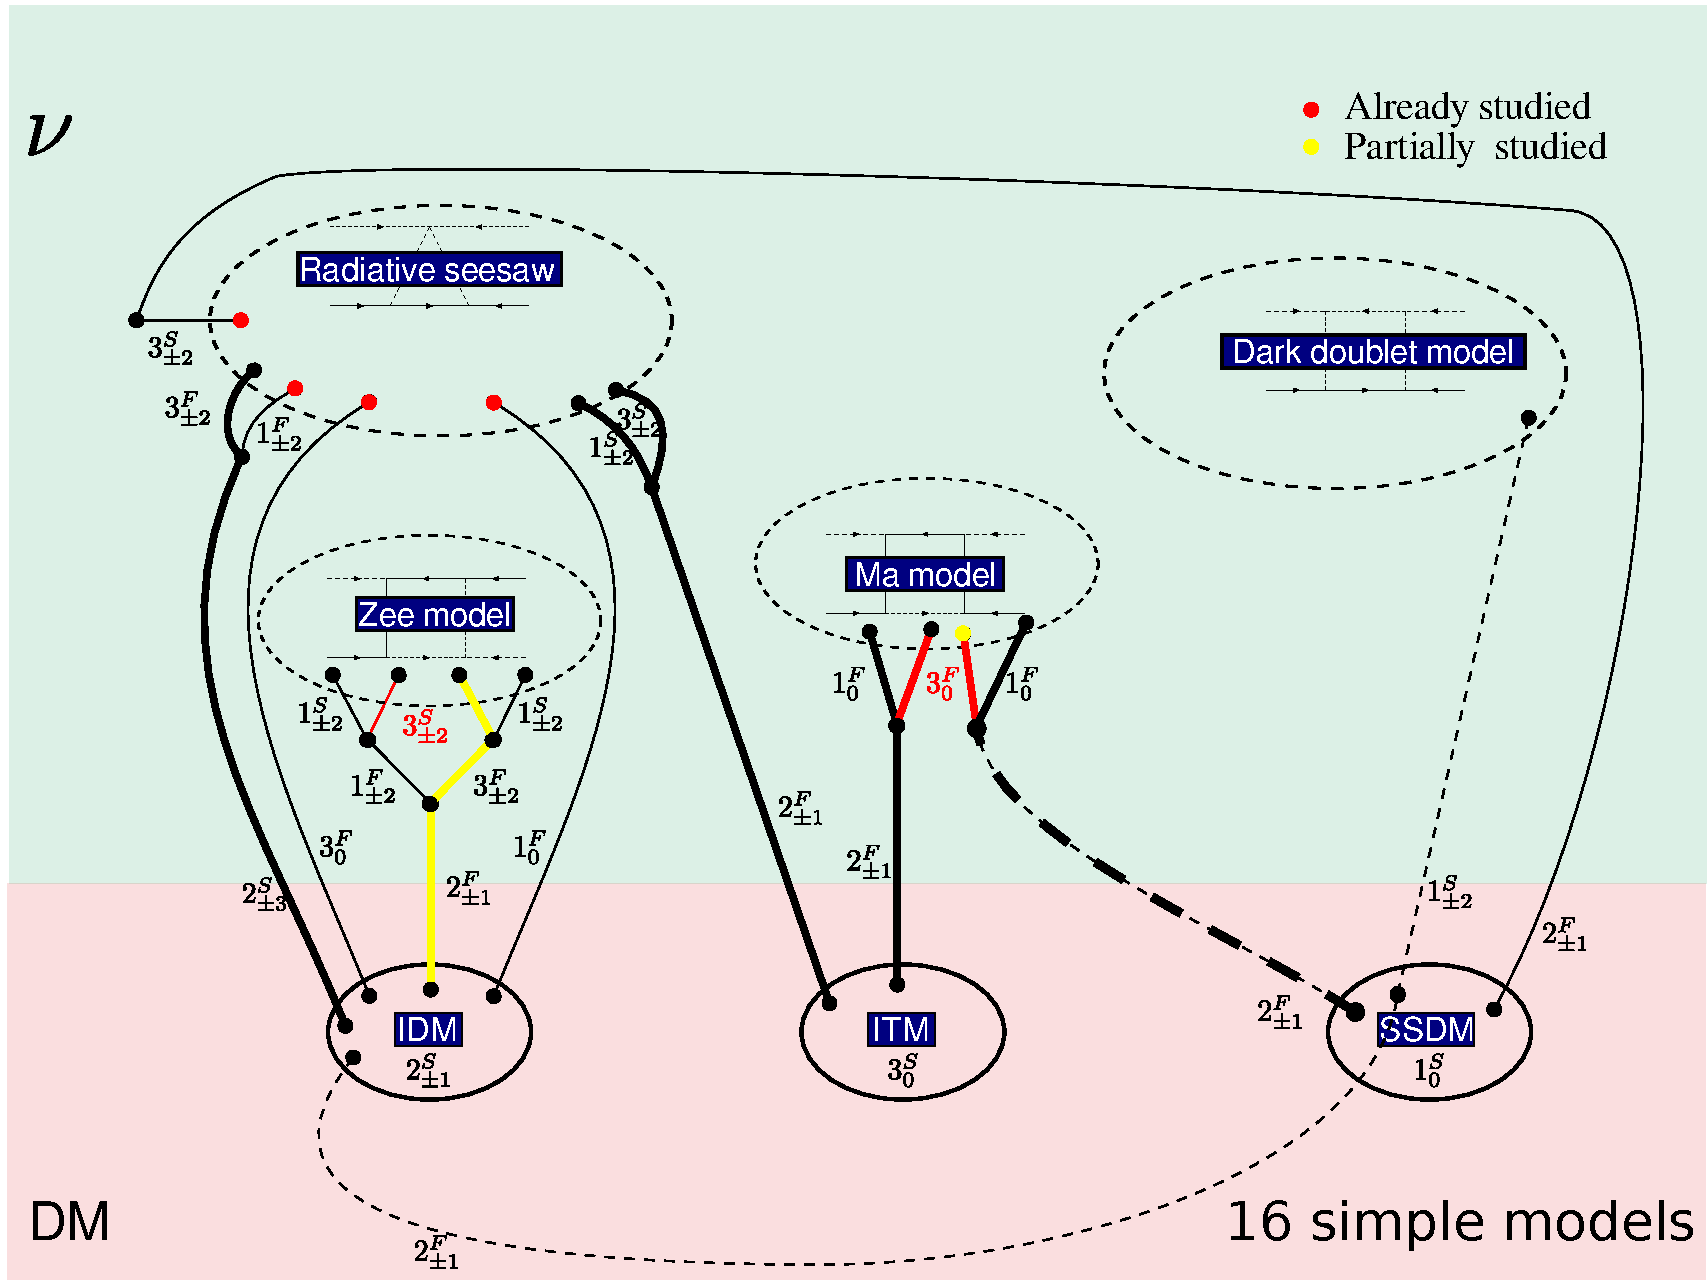
\includegraphics[width=\paperwidth,height=\paperheight]{dmwmodels8}}}%
\only<9>{\put(-12,-13){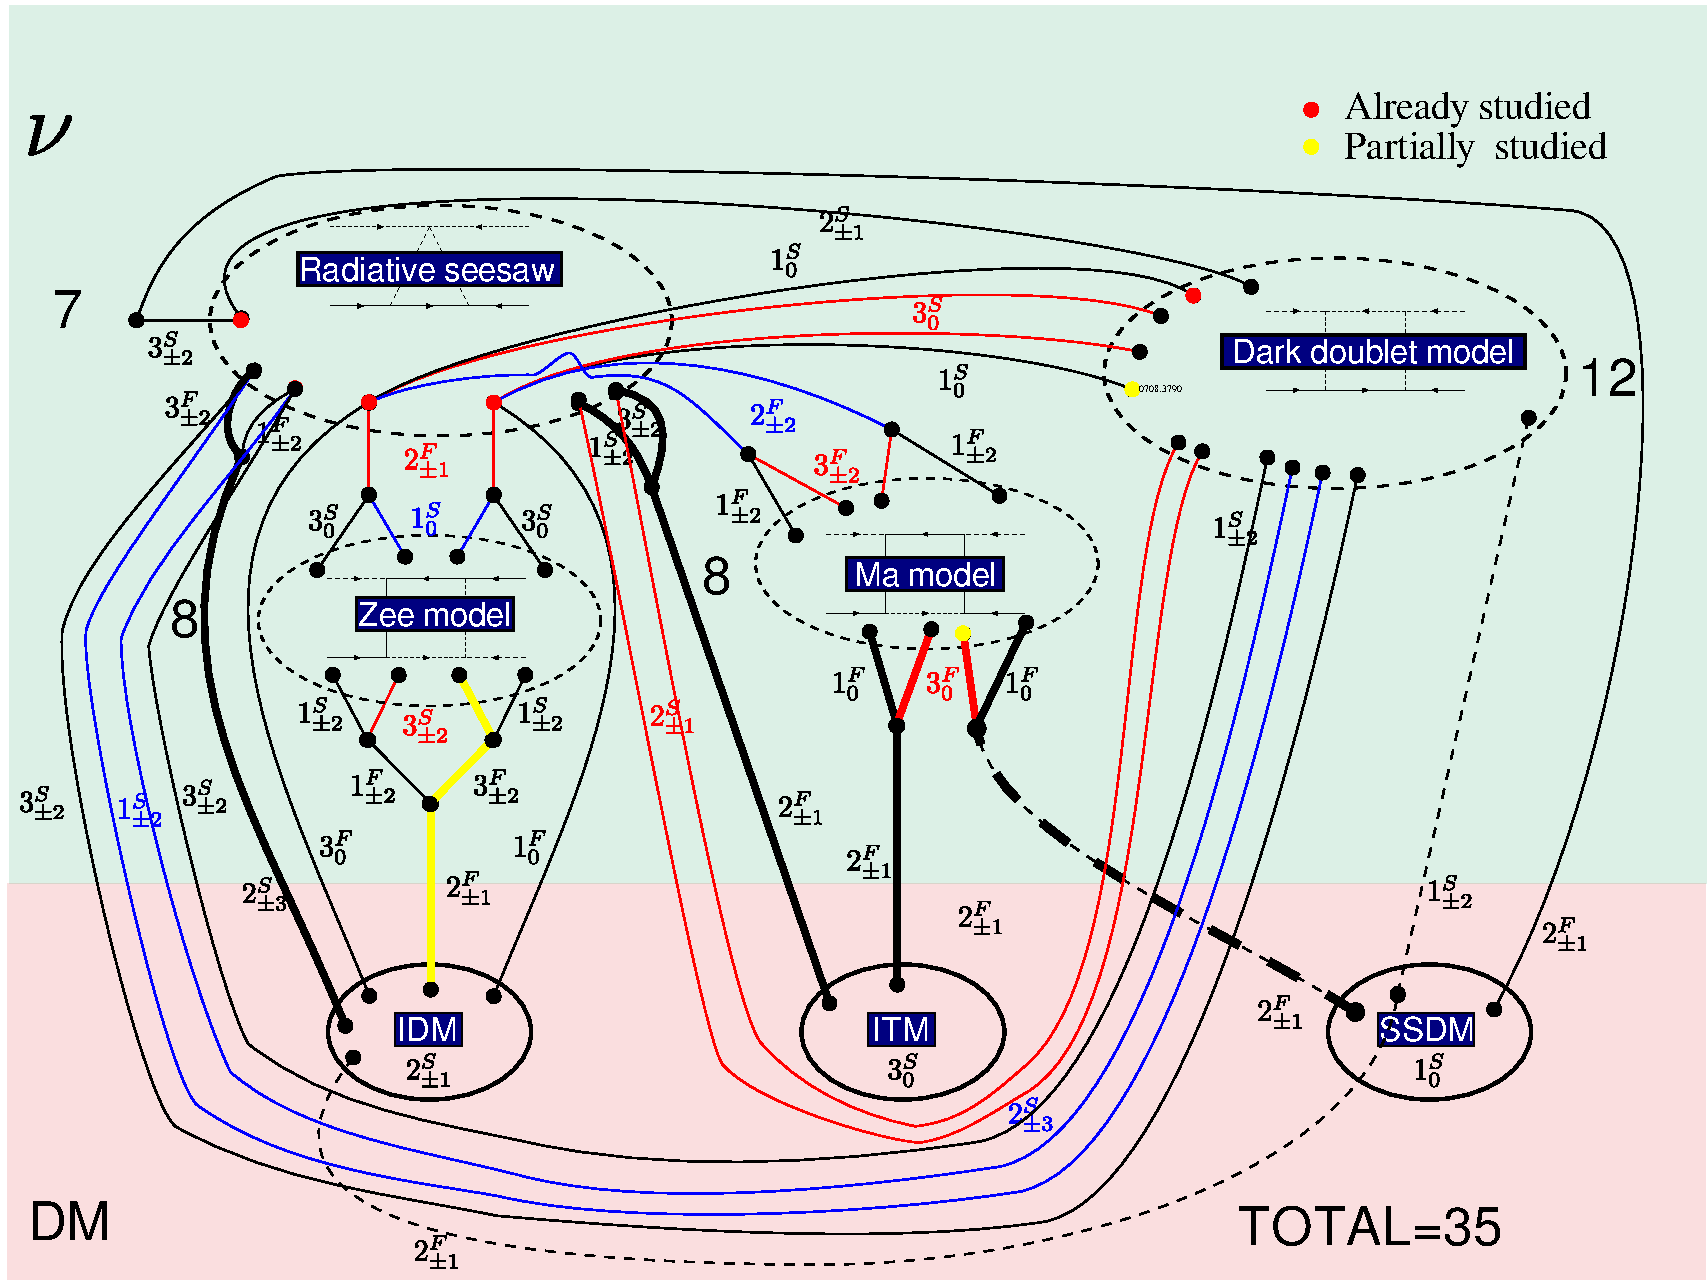
\includegraphics[width=\paperwidth,height=\paperheight]{dmwmodels9}}}%
\only<10>{\put(-12,-13){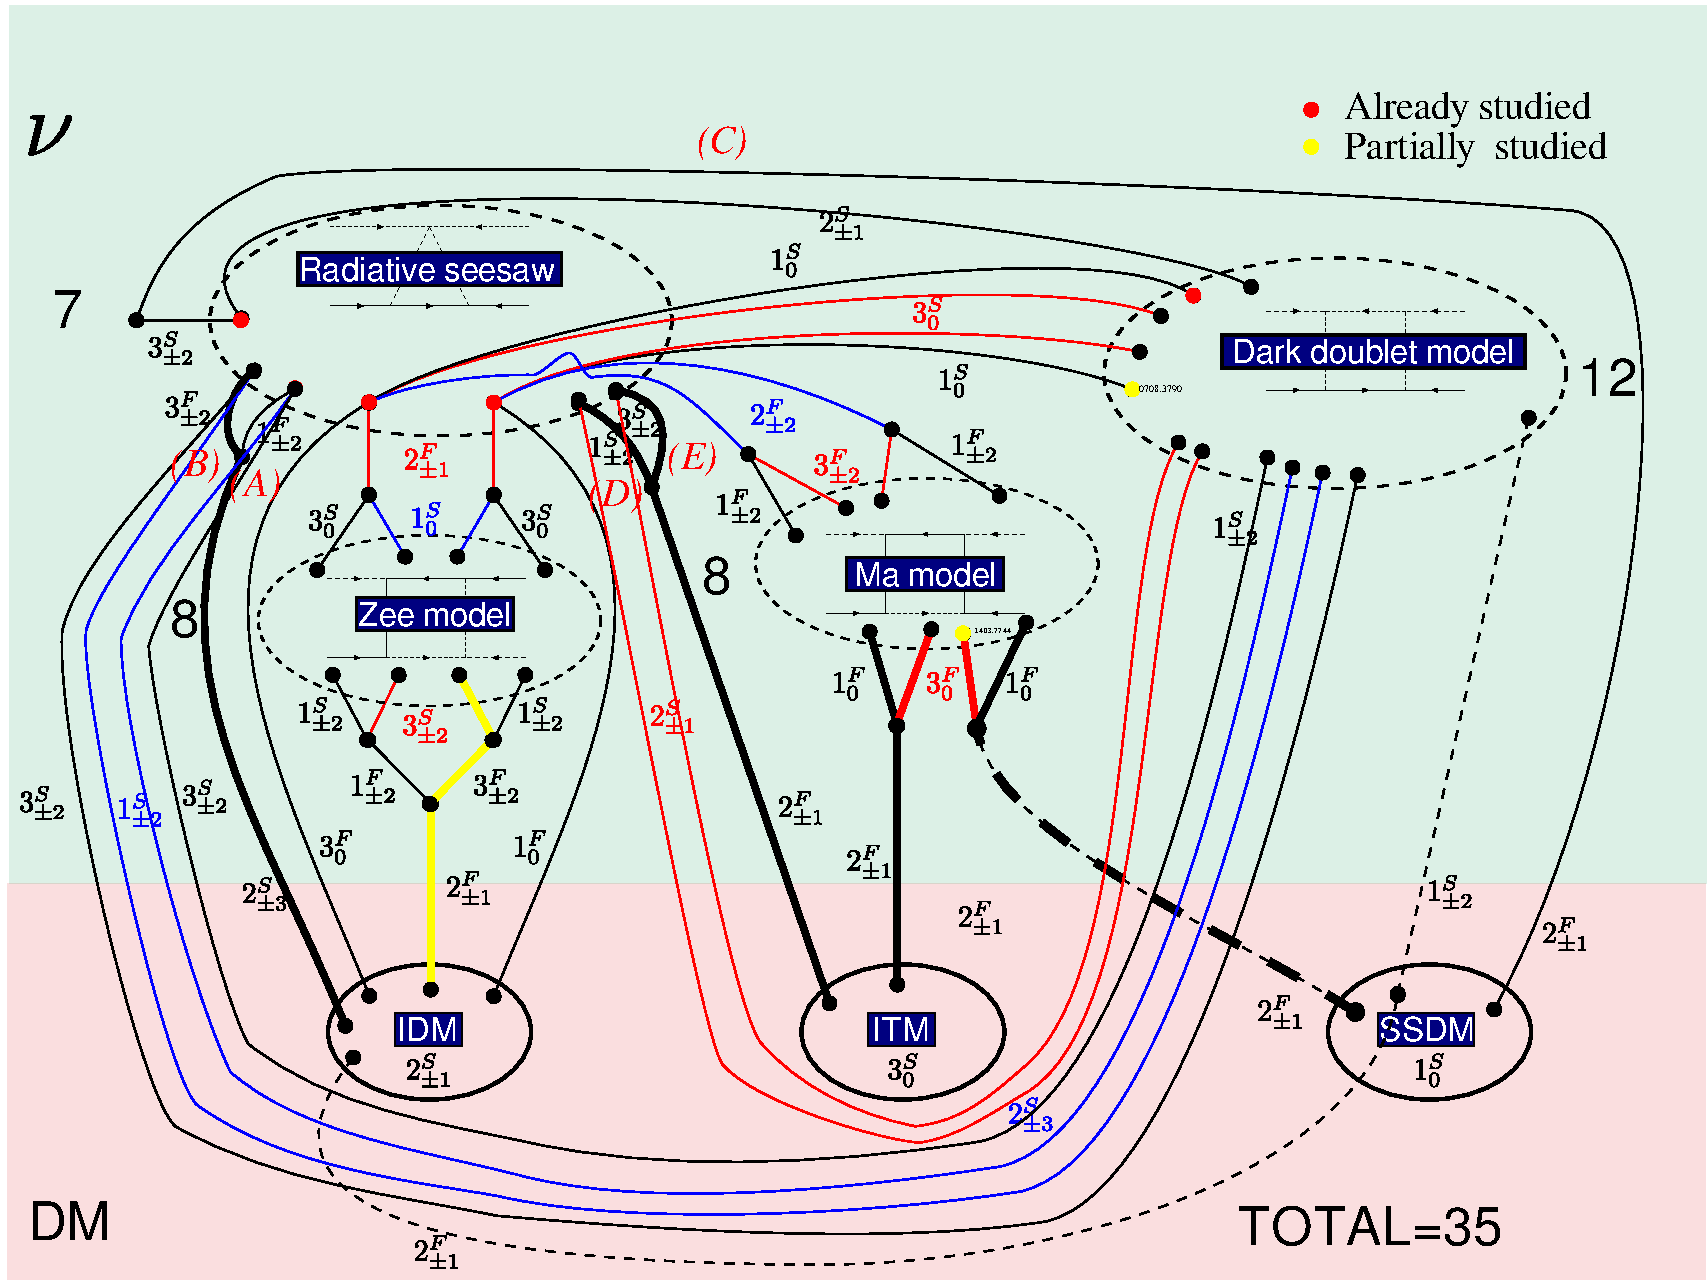
\includegraphics[width=\paperwidth,height=\paperheight]{dmwmodels10}}}%
\only<10>{\put(40,240){\begin{beamercolorbox}[sep=0.01em,wd=5.7cm,center,rounded=true,shadow=true]{cite}
\scriptsize Law, McDonald, arXiv:1305.6467
\end{beamercolorbox}}}
\end{picture}
\end{frame}
%%%%%%%%%%%%%%%%%%%%%%%
\begin{frame}
\begin{picture}(320,250)
\only<1>{\put(-10,98){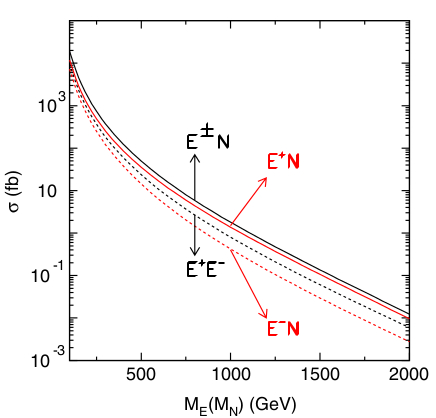
\includegraphics[scale=0.5]{09074193}}}%
\only<1>{\put(20,238){\small arXiv:0907.4193:  $3^{F}_{0}$}}%
\only<1>{\put(150,98){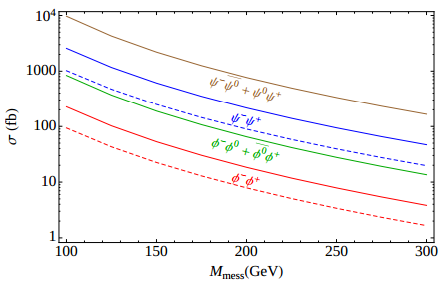
\includegraphics[scale=0.6]{13034404}}}%
\only<1>{\put(160,238){\small arXiv:1303.4404:  $2^{F,S}_{\pm 1}$ (solid) $1^{F,S}_{\pm 2}$ (dashed)}}%
\only<1>{\put(100,-20){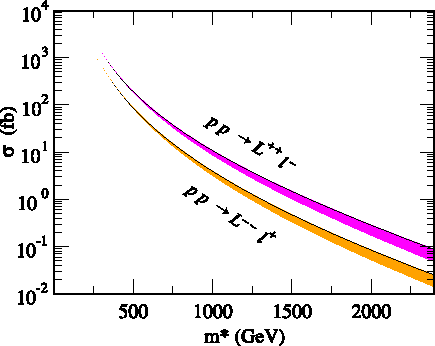
\includegraphics[scale=0.72]{12013764}}}%
\only<1>{\put(10,40){\small arXiv:1201.3764  $3^{F}_{\pm 2}$}}%

\end{picture}
\end{frame}
%%%%%%%%%%%%%%%%
\begin{frame}
\begin{picture}(320,250)
\only<1>{\put(-10,70){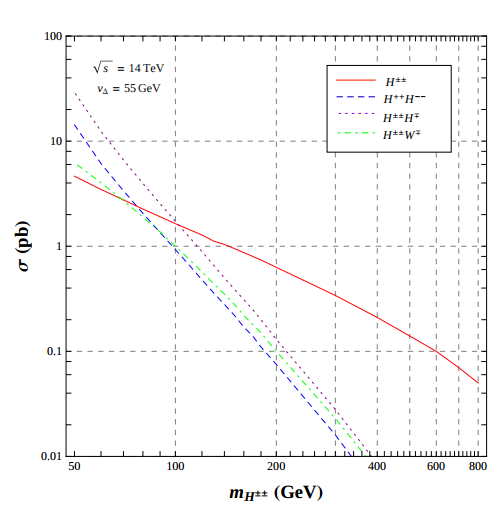
\includegraphics[scale=0.5]{12022014}}}%
\only<1>{\put(20,60){\small arXiv:1202.2014:  $3^{S}_{\pm 2}$}}%
\only<1>{\put(150,0){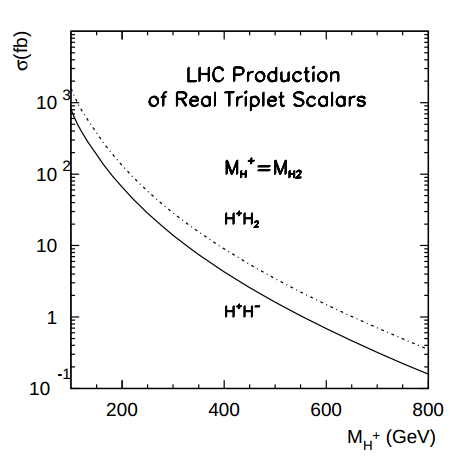
\includegraphics[scale=0.6]{08113957}}}%
\only<1>{\put(180,0){\small arXiv:0811.3957:  $3^{S}_{0}$}}%

\end{picture}
\end{frame}

%\begin{frame}
%Phys Rev D85 095018
%\begin{picture}(320,250)
%\only<1>{\put(-10,70){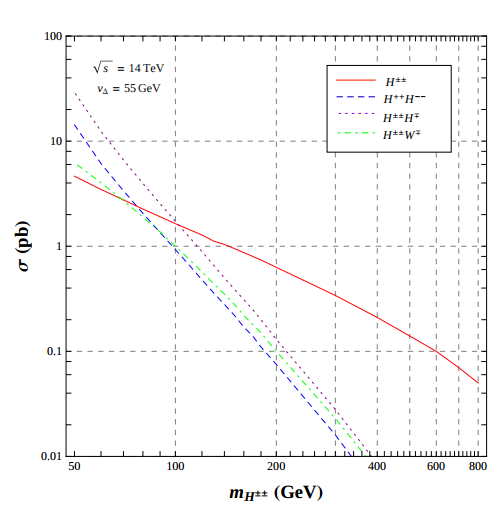
\includegraphics[scale=0.5]{12022014}}}%
%\only<1>{\put(20,40){\small arXiv:1202.2014:  $3^{S}_{\pm 2}$}}%
%\end{picture}
%\end{frame}



%%%%%%%%%%%
\begin{frame}
  \frametitle{Discussion}

\includegraphics[scale=0.6]{alg}
  \begin{itemize}
  \item The collider and dark matter phenomenology  of many of these viable models have yet to be studied in detail.
  \item We have only qualitatively described the particle content and the dark matter candidates of each model. A more specific analysis of some of these models is certainly desirable.
\item Some strategies to systematically search for this kind of models
  at colliders would be designed. 
  \item New particles allowed to be even under $Z_2$ could give rise to new possibilities.
  \end{itemize}
\end{frame}
%%%%%%%%%%%%%%%%5


\end{document}





TEMPLATES

1. Background image slide
%%%%%%%%%%%%%%%%%%%%%%%%%%%%%%
{
\usebackgroundtemplate{\includegraphics[width=\paperwidth]{file}}
\setbeamertemplate{blocks}[rounded][shadow=false]
\setbeamercovered{invisible}
\begin{frame}[plain]
\end{frame}
}
%%%%%%%%%%%%%%%%%%%%%%%%%%%%%%

2. Two columns
\begin{columns}
  \column{.48\textwidth}
  \begin{block}<2->{}
  \end{block}
  \column{.48\textwidth}
  \begin{block}<2->{}
  \end{block}
\end{columns}

%%%%%%%%%%%%%%%%%%%%%
{
\usebackgroundtemplate{\includegraphics[width=\paperwidth]{file}}
\setbeamertemplate{blocks}[rounded][shadow=false]
\setbeamercovered{invisible}
\begin{frame}[plain]
  \begin{block}{}
    Name
  \end{block}
\end{frame}
}
%%%%
{
\usebackgroundtemplate{\includegraphics[width=\paperwidth]{file}}
\setbeamertemplate{blocks}[rounded][shadow=false]
\setbeamercovered{invisible}
\begin{frame}[plain]
\end{frame}
%%%%%%%%%%%%%%%%%%
}


%Trick to put stuff in specfic places of an slide:
\begin{frame}
\begin{picture}(320,250)
\put(-25,190){D.R. \emph{et al}: arXiv:1006.5075 [PRD]\qquad\qquad arXiv:1206.3605 [PRD]}
\put(-37,20){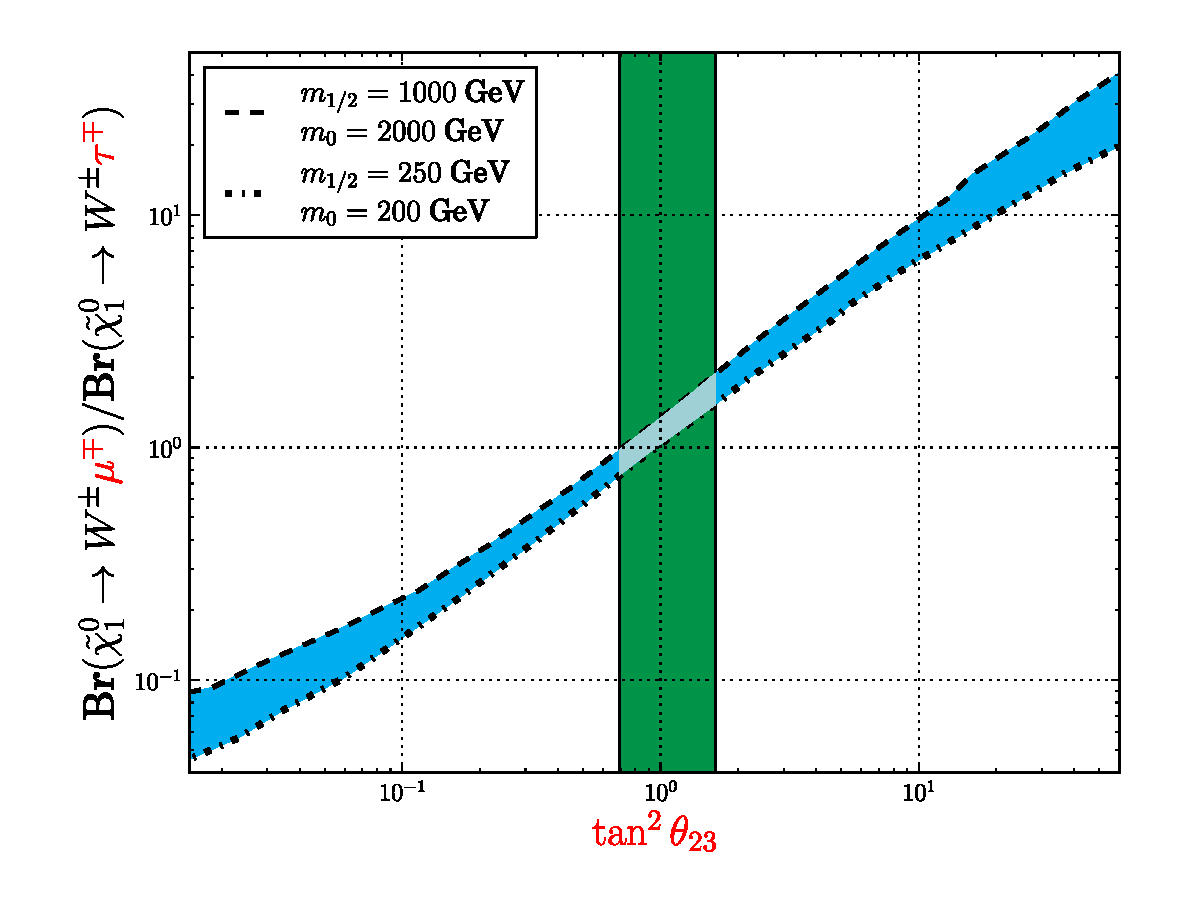
\includegraphics[scale=0.35]{atmcorrelationm}}
\put(143,20){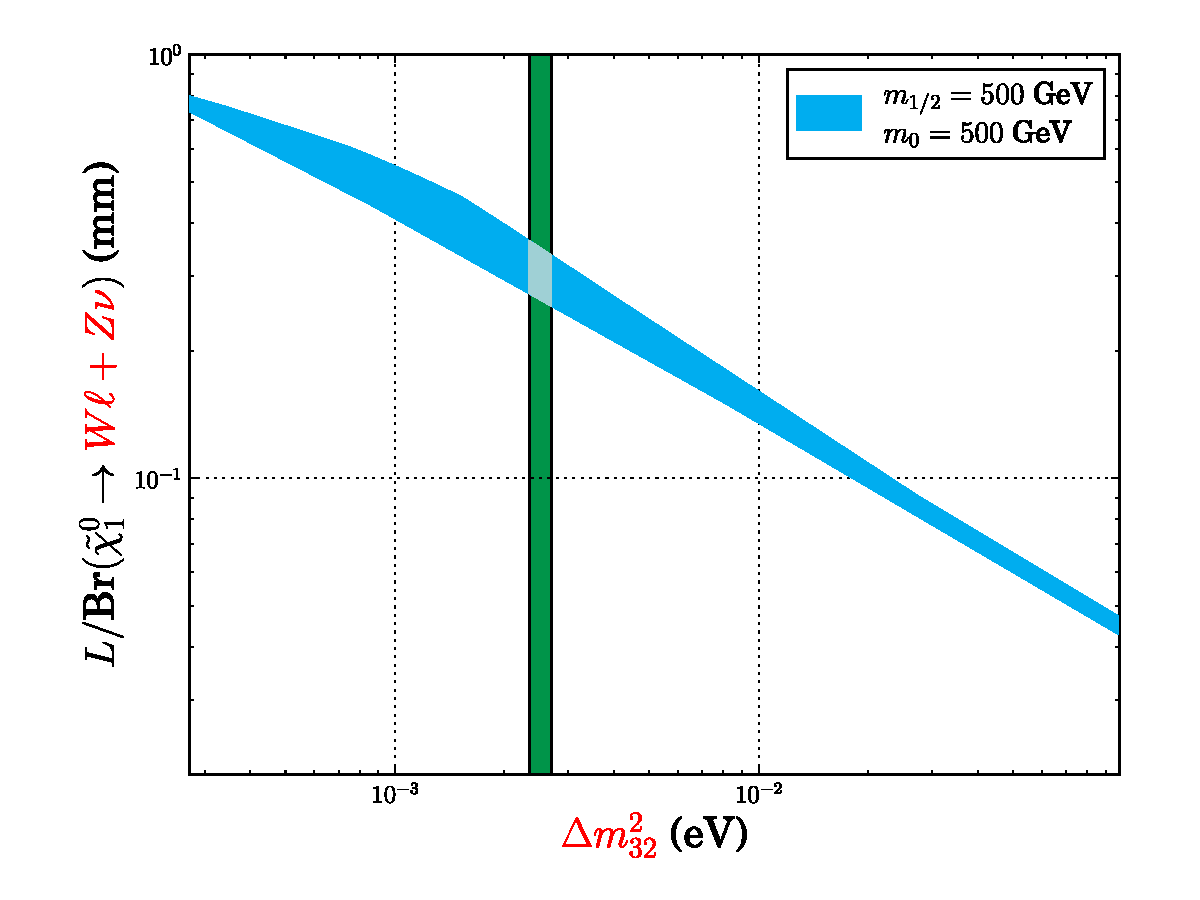
\includegraphics[scale=0.35]{LoverWlZnu_Dm23_500_500_randomm}}
\put(0,160){Only depend in \alert{$\Lambda_i$}}
\end{picture}
\end{frame}
%%%%%
Background like
%%%%%%%%%%%%%%%%%%%%%%%%
\begin{frame}[plain]
\begin{picture}(320,250)
\only<1>{\put(-30,-15){\includegraphics[width=\paperwidth]{brpv1}}}%
\only<2>{\put(-30,-15){\includegraphics[width=\paperwidth]{brpv2}}}%    
\only<2>{\put(-30,-15){\includegraphics[width=\paperwidth]{brpv3}}}%    
\end{picture}
\end{frame}


%%%
Post it

\setbeamercolor{postit}{fg=black,bg=yellow}
\begin{beamercolorbox}[sep=1em,wd=5cm]{postit}
Place me somewhere!
\end{beamercolorbox}

%%%combine with textblock
\begin{textblock*}{297mm}(0mm,0mm)%
\begin{beamercolorbox}[sep=0.1em,wd=4cm,center,rounded=true,shadow=true]{cite}
\scriptsize Akhmedov, hep-ph/0001264
\end{beamercolorbox}
\end{textblock*}

%%More colorboxes
\setlength{\fboxrule}{3 pt}
\fcolorbox{red}{yellow}{caja de fondo
amarillo y contorno rojo}\\
\setlength{\fboxsep}{5pt}
\fcolorbox{red}{yellow}{caja de fondo
amarillo y contorno rojo}